\documentclass[10pt,a4paper,twoside,openright]{book}

% contenuto identico a template_dispense.tex
\input{style.tex}
\usepackage{pifont}
\newcommand{\cmark}{\ding{51}}%
\newcommand{\xmark}{\ding{55}}%
\usepackage{pdfpages}

\usepackage{geometry}
\geometry{
	nomarginpar, % Toglie doppi margini
	margin=1in, % Imposta i margini a 1 inch
}

% Comandi pratici

% Lettere comuni in grassetto
\newcommand{\x}{\mathbf{x}}
\newcommand{\y}{\mathbf{y}}
\newcommand{\zer}{\mathbf{0}}

% Lettere comuni in grassetto greche
\usepackage{bm} % per avere le lettere greche in bold con \bm{\sigma}
\newcommand{\sigg}{\bm{\sigma}}
\newcommand{\nuu}{\bm{\nu}}
\newcommand{\alphaa}{\bm{\alpha}}

% d nell'integrale e i rispettivi usi
\newcommand{\de}{\,\mathrm d}
\newcommand{\dx}{\de x}
\newcommand{\dy}{\de y}
\newcommand{\dl}{\de l}
\newcommand{\dr}{\de r}
\newcommand{\ds}{\de s}
\newcommand{\dt}{\de t}
\newcommand{\dv}{\de v}
\newcommand{\dxi}{\de \xi}
\newcommand{\drho}{\de \rho}

% d nell'integrale con differenziale vettoriale
\newcommand{\dxx}{\de \x}
\newcommand{\dyy}{\de \y}
\newcommand{\dsig}{\de \sigg}

\newcounter{es}
\newcommand{\Es}{
	\stepcounter{es}
	\section{Esercizio \arabic{es}}
	}
\numberwithin{es}{chapter}

\newcommand{\Par}{\textbf{Parametri}}
\newcommand{\Var}{\textbf{Variabili}}
\newcommand{\Fob}{\textbf{Funzione obiettivo}}
\newcommand{\Vin}{\textbf{Vincoli}}

% Non servono, preferisco la numerazione locale e non globale delle figure e delle equazioni
%\usepackage{chngcntr}
%\counterwithout{figure}{chapter}
%\counterwithout{equation}{chapter}

\allowdisplaybreaks[4] % Consente di rompere equazioni su più pagine

%%%%%%%%%%%%%%%%%%%%%%%%%%%%%%%%%%%%%%%%%%%%%%%
%%%%%%%%%%%%%%%%%%%%%%%%%%%%%%%%%%%%%%%%%%%%%%%

\begin{document}

%%%%%%%%%%%%%%%%%%%%%%%%%%%%%%%%%%%%%%%%%%%%%%%
%%%%%%%%%%%%%%%%%%%%%%%%%%%%%%%%%%%%%%%%%%%%%%%

\frontmatter
\pagestyle{empty} % SWITCHA PER NON AVERE NUMERO PAGINA
\vspace*{\fill}
\begin{center}
	{\large \textsc{Soluzioni agli esercizi aggiuntivi di}}\\
	\vspace*{0.4cm}
	{\Huge \textsc{Fondamenti di Ricerca Operativa}}\\
	\vspace*{1cm}
	{\large {di Teo Bucci e Filippo Cipriani}}\\
	\vspace*{1cm}
	Politecnico di Milano\\A.A. 2020/2021\\
	\vspace*{1cm}
	Revisione del 2 Febbraio 2022
\end{center}
\vspace*{\fill}
\newpage

%%%%%%%%%%%%%%%%%%%%%%%%%%%%%%%%%%%%%%%%%%%%%%%
%%%%%%%%%%%%%%%%%%%%%%%%%%%%%%%%%%%%%%%%%%%%%%%

%{\Large \textit{Appunti di Equazioni alle Derivate Parziali}}
%
%\vspace*{\fill}
%
%\textcopyright \ Gli autori, tutti i diritti riservati
%
%Sono proibite tutte le riproduzioni senza autorizzazione scritta degli autori.
%
%Revisione del \today
%
%Developed by\\
%Teo Bucci - \texttt{teobucci8@gmail.com}\\
%Filippo Cipriani - \texttt{filippo.cipriani99@hotmail.it}\\ \\
%Compiled with \ensuremath\heartsuit \\

%\textbf{Prefazione}

%Per segnalare eventuali errori o suggerimenti potete contattare gli autori.

\newpage

%%%%%%%%%%%%%%%%%%%%%%%%%%%%%%%%%%%%%%%%%%%%%%%
%%%%%%%%%%%%%%%%%%%%%%%%%%%%%%%%%%%%%%%%%%%%%%%

% INDICE
\addtocontents{toc}{\protect\thispagestyle{empty}}
\tableofcontents
%\newpage

%%%%%%%%%%%%%%%%%%%%%%%%%%%%%%%%%%%%%%%%%%%%%%%
%%%%%%%%%%%%%%%%%%%%%%%%%%%%%%%%%%%%%%%%%%%%%%%

% PAGINA VUOTA PER FAR PARTIRE IL CAPITOLO IN UNA PAGINA DISPARI
%\myNewEmptyPage

\AtEndDocument{\cleardoublepage}

%%%%%%%%%%%%%%%%%%%%%%%%%%%%%%%%%%%%%%%%%%%%%%%
%%%%%%%%%%%%%%%%%%%%%%%%%%%%%%%%%%%%%%%%%%%%%%%

\mainmatter
\pagestyle{fancy} % Riswitcha per riavere il numero pagina
%\setcounter{page}{1} % Fa ripartire il contatore pagina da 1

%%%%%%%%%%%%%%%%%%%%%%%%%%%%%%%%%%%%%%%%%%%%%%%
%%%%%%%%%%%%%%%%%%%%%%%%%%%%%%%%%%%%%%%%%%%%%%%

%!TEX root = ../fro.tex
\chapter{Programmazione Lineare}

\Es

\Par

$P$ porti, $i=1,2,3$

$c_{i}$ costo per porto per ogni vettura $( 150,250,200)$

$t_{i}$ costo fisso porto

$S$ centri di smistamento, $j=1,\dotsc ,4$

$k_{i}$ costo di invio dal porto $i$ al km

$a_{ij}$ distanza dal porto $i$ al centro $j$

$r_{j}$ richiesta del centro $j$

$d_{i}$ capacità del porto $i$

\Var

$x_{ij} \geq 0,x_{ij} \in \mathbb{Z}$ numero di automobili dal porto $i$ al centro $j$

$y_{i} \in \{0,1\}$, uguali a $1$ se uso il porto $i$

$z_{ij} \in \{0,1\}$, uguali a $1$ se il porto $i$ rifornisce il centro $j$

\Fob

\begin{equation*}
	\min\bigg\{\underbrace{\sum _{ij} c_{i} x_{ij}}_{\text{auto}} +\underbrace{\sum _{i} t_{i} y_{i}}_{\text{porto}} +\underbrace{\sum _{ij} a_{ij} k_{i} x_{ij}}_{\text{trasporto}}\bigg\}
\end{equation*}

\Vin

\begin{align*}
	\sum _{i} x_{ij} &\geq r_{j} \qquad\forall j\in S && \text{richiesta}\\
	\sum _{j} x_{ij} &\leq d_{i} y_{i} \qquad\forall i\in P && \text{bigM + capacità}\\
	\sum _{i} z_{i,3} &=1 && \text{centro 3}\\
	x_{ij} &\leq d_{i} z_{ij} \qquad\forall i\in P,\forall j\in S && \text{bigM}\\
	z_{22} &\leq z_{24} && \text{logico}\\
\end{align*}

\Es

\Par

$A$ aeroporti

$H$ hangar

$c_{j},s_{j},t_{j}$ operatori $\forall j\in H$

$g_{1}$ costo squadra $1$

$g_{2}$ costo squadra $2$

$g_{3}$ costo squadra $3$

\begin{center}
	
	\begin{tabular}{|c|c|c|}
		\hline 
		$1$c & $1$s & $1$t \\
		\hline 
		$3$c & $1$s & X    \\
		\hline 
		$3$c & $2$s & $2$t \\
		\hline
	\end{tabular}
\end{center}

\Var

$x_{j} \geq 0,x_{j} \in \mathbb{Z}$ squadre tipo $1$

$y_{j} \geq 0,y_{j} \in \mathbb{Z}$ squadre tipo $2$

$z_{j} \geq 0,z_{j} \in \mathbb{Z}$ squadre tipo $3$

$\varphi \in \{0,1\}$, uguale a $1$ se uso 3 squadre di tipo $2$

$w_{ij} \in \{0,1\}$, uguale a $1$ se aereo $i$ in hangar $j$, $\forall i\in A,\forall j\in H$

\Fob

\begin{equation*}
	\min \sum _{j}( x_{j} g_{1} +y_{j} g_{2} +z_{j} g_{3})
\end{equation*}

\Vin

\begin{align*}
	\sum _{j} w_{ij} &=1\qquad\forall i\in A&&\text{assegnazione}\\
	x_{j} +3y_{j} +3z_{j} &\geq \sum _{i} c_{j} w_{ij} \qquad\forall j\in H &&\text{operai}\\
	x_{j} +\phantom{3}y_{j}  +2z_{j} &\geq \sum _{i} s_{j} w_{ij} \qquad\forall j\in H &&\text{operai}\\
	x_{j} \phantom{+3y_{j}}  +\phantom{2}z_{j}  &\geq \sum _{i} t_{j} w_{ij} \qquad\forall j\in H &&\text{operai}\\
	\sum _{j} y_{j} -2&\leq M\varphi &&\text{(A)}\\
	2\varphi &\leq \sum _{j} z_{j}&&\text{(B)}
\end{align*}

Gli ultimi due vincoli servono per realizzare:
\begin{equation*}
	y_{j} \geq 3\ \ \overset{\text{(A)}}{\Rightarrow } \ \ \varphi =1\ \ \overset{\text{(B)}}{\Rightarrow } \ \ z_{j} \geq 2
\end{equation*}

\Es

\Par

$p_{j} ,\ j=1,2$

$r_{j}$ prezzo vendita

$d_{j}$ domanda

$I$ materie prime $i\in I$

$c_{i}$ disponibilità

$g_{i}$ costo unitario materie prima

$g_{ji}$ materia $i$ necessaria per $j$

$o_{1}$ ore $p_{1}$ da materia prima

$o_{2}$ ore $p_{2}$ da materia prima

oppure ottengo $p_{2}$ con

$b$ unità di $p_{1}$ per $p_{2}$

$o_{3}$ ore lavorazione ($p_{2}$ da $p_{1}$)

$k$ costo fisso attivazione

$O$ ore a disposizione

\Var

$x_{j} \geq 0,x_{j} \in \mathbb{Z}$ unità di prodotto $j$ da materie prime

$y\geq 0,y\in \mathbb{Z}$ unità di prodotto $2$ da prodotto $1$

$z\in \{0,1\}$, uguale a $1$ se attivo processo produttivo

\Fob

\begin{equation*}
	\max\left\{[ r_{1}( x_{1} -by) +r_{2}( x_{2} +y)] -\left[\sum _{ij} g_{i} q_{ji} x_{j} +kz\right]\right\}
\end{equation*}

\Vin

\begin{align*}
	y&\leq Mz && \text{bigM}\\
	( x_{1} -by) &\geq d_{1} && \text{richiesta}\\
	( x_{2} -y) &\geq d_{2} && \text{richiesta}\\
	\sum _{j} q_{ji} x_{j} &\leq c_{i} \qquad\forall i\in I && \text{disponibilità}\\
	o_{1} x_{1} +o_{2} x_{2} +o_{3} y&\leq O && \text{disponibilità}\\
\end{align*}

\Es

\Par

$T$ gruppi $i\in T$

$p_{i}$ persone

$J$ aerei $j\in J$

$c_{j}$ costo noleggio

$B_{j}$ capienza aereo

$A$ aeroporto $k\in A$

$G_{k}$ max voli per aeroporto

$l_{jk}$ costo di far partire $j$ da $k$

$R$ sottoinsiemi di aeroporti vicini

$S_{r}$ con $r=1,\dotsc ,R$, al più un aeroporto

\Var

$x_{ij} \in \{0,1\}$, uguale a $1$ se gruppo $i$ ad aereo $j$

$y_{jk} \in \{0,1\}$, uguale a $1$ se aereo $j$ parte da $k$

$z_{j} \in \{0,1\}$, uguale a $1$ se uso aereo $j$

$w_{k} \in \{0,1\}$, uguale a $1$ se uso aeroporto $k$

\Fob

\begin{equation*}
	\min\left\{\sum _{j} c_{j} z_{j} +\sum _{jk} l_{jk} y_{jk}\right\}
\end{equation*}

\Vin

\begin{align*}
	\sum _{i} x_{ij} &\leq Mz_{j} \qquad\forall j\in J && \text{bigM} \\
	\sum _{i} p_{i} x_{ij} &\leq B_{j} \qquad\forall j\in J && \text{capacità} \\
	\sum _{j} y_{jk} &\leq G_{k} w_{k} \qquad\forall k\in K && \text{bigM + capienza voli} \\
	\sum _{k\in S_{r}} w_{k} &\leq 1\qquad\forall r=1,\dotsc ,R && \text{no aeroporti vicini} \\
	\sum _{j} x_{ij} &=1\qquad\forall i\in I && \text{assegnamento} \\
	\sum _{k} y_{jk} &=z_{j} \qquad\forall j\in J && \text{un aereo per aeroporto, se usato} \\
\end{align*}

\Es

\Par

$P$ domande iscrizione $i\in P$

$M\subset P,F\subset P$, uomini, donne $( M\cup F=P,M\cap F=\emptyset )$

$n$ max persone per classe

$d$ massimo classi ($D=1,\dotsc ,d$ insieme classi)

$b_{i}$ preparazione di $i$

$q$ livello minimo per classe

$C$ coppie formate $( i,j) \in C,i\in M,j\in F$

\Var

$x_{ik} \in \{0,1\}$, uguale a $1$ se persona $i$ in classe $k$

$y_{i} \in \{0,1\}$, uguale a $1$ se accetto domanda

\Fob

\begin{equation*}
	\max\sum _{i} y_{i}
\end{equation*}

\Vin

\begin{align*}
	\sum _{i\in P} x_{ik} &\leq n\qquad\forall k\in D && \text{capacità classe} \\
	\sum _{i\in M} x_{ik} &=\sum _{i\in F} x_{ik} \qquad\forall k\in D && \text{uguali $M/F$} \\
	\sum _{i\in P} x_{ik} b_{i} &\geq q\sum _{i\in P} x_{ik} \qquad\forall k\in D && \text{preparazione} \\
	y_{i} &\leq \sum _{k\in D} x_{ik} \qquad\forall i\in P && \text{bigM} \\
	\sum _{k\in D} x_{ik} &\leq 1\qquad\forall i\in P && \text{massimo $1$ corso per persona} \\
	x_{ik} &=x_{jk} \qquad\forall (i,j)\in C,\forall k\in D && \text{coppie} \\
\end{align*}

\Es

\Par

$A$ insieme altiforni $i=1\dotsc N,i\in A$

$m_{i}$ max quintali per altiforno

$P$ prodotti $j\in P$

$q_{1j}$ prodotto $j$ da 1 quintale di materia prime con processo 1 (prodotto/quintale)

$q_{2j}$ prodotto $j$ da 1 quintale di materia prime con processo 2 (prodotto/quintale)

$r_{j}$ richiesto prodotto

$c_{1i}$ costo lavorazione al quintale in altiforno $i$ con processo 1 (euro/quintale)

$c_{2i}$ costo lavorazione al quintale in altiforno $i$ con processo $2$ (euro/quintale)

$f_{i}$ costo attivazione processo 2 in altiforno $i$

\Var

$w_{i} \in \{0,1\}$, uguale a $1$ se lavoro più di $q$

$y_{i} \in \{0,1\}$, uguale a $1$ se uso processo $2$

$x_{ij1} \geq 0,x_{ij1} \in \mathbb{Z}$ prodotto $j$ con processo $1$ in altiforno $i$

$x_{ij2} \geq 0,x_{ij2} \in \mathbb{Z}$ prodotto $j$ con processo $2$ in altiforno $i$

\Fob

\begin{equation*}
	\min \left\{\sum _{i} y_{i} f_{i} +\sum _{ij}\left[ c_{1i}\frac{x_{ij1}}{q_{1j}} +c_{2i}\frac{x_{ij2}}{q_{2j}}\right]\right\}
\end{equation*}

\Vin

\begin{align*}
	\sum _{j} x_{ij2} & \leq My_{i} \qquad\forall i\in A && \text{bigM} \\
	\sum _{j}\left[\frac{x_{ij1}}{q_{1j}} +\frac{x_{ij2}}{q_{2j}}\right] & \leq m_{i} \qquad\forall i\in A && \text{capacità} \\
	\sum _{i}[ x_{ij1} +x_{ij2}] & \geq r_{j} \qquad\forall j\in P && \text{richiesta} \\
	\sum _{i} y_{i} & \leq N-1 && \text{no processo $2$ su tutti gli altiforni} \\
	\sum _{i} w_{i} & \geq 1 && \text{almeno 1 usa più di $q$ quintali} \\
	qw_{i} & \leq \sum _{ij}\left[\frac{x_{ij1}}{q_{1j}} +\frac{x_{ij2}}{q_{2j}}\right] \qquad\forall i\in A && \text{vincolo logico} \\
\end{align*}

\Es

\Par

$C$ cioccolatini $i\in C$

$S$ confezioni regalo $j\in S$

$r_{ij}$ richieste cioccolatini $i$ in confezione $j$

$g_{i}$ costo cioccolatino

$m_{i}$ max produzione

$p_{i}$ vendita cioccolatino sfuso $i$

$d_{j}$ vendita confezione $j$

$b_{j}$ costo scatola $j$

\Var

$x_{i} \geq 0,x_{i} \in \mathbb{Z}$ numero cioccolatini $i$ prodotti

$y_{j} \geq 0,y_{j} \in \mathbb{Z}$ numero confezioni $j$ prodotte

$z\in \{0,1\}$, uguale a $1$ se acquisto almeno $q$ scatole

\Fob

\begin{equation*}
	\max\bigg\{\underbrace{\sum _{j} d_{j} y_{j}}_{\text{confezioni}} +\underbrace{\sum _{i} p_{i}\bigg( x_{i} -\sum _{j} r_{ij} y_{j}\bigg)}_{\text{sfusi}} -\underbrace{\sum _{i} g_{i} x_{i}}_{\text{costo prod.}} -\underbrace{\sum _{j} b_{j} y_{j}}_{\text{costo scatole}} +\underbrace{zB}_{\text{sconto}}\bigg\}
\end{equation*}

\Vin

\begin{align*}
	x_{i} & \geq \sum _{j} r_{ij} y_{j} \qquad\forall i\in I && \text{richiesta} \\
	x_{i} & \leq m_{i} \qquad\forall i\in I && \text{capacità} \\
	\sum _{j} y_{j} & \geq Qz && \text{sconto} \\
	x_{1} & \geq 0.2\cdot \sum _{i} x_{i} && \text{qualità} \\
\end{align*}

\Es

\Par

$D$ difensori

$A$ attaccanti

$G$ giocatori $i\in G$

$r_{i} \in \{0,1\}$, uguale a $1$ se giocatore $i$ è attaccante

$v_{i}$ valore giocatore

$B$ valore complessivo formazione

$q$ giocatori non giocanti

$K$ formazioni $|K|=2$

\Var

$z\geq 0,z\in \mathbb{Z}$ valore formazione di minimo valore

$x_{ik} \in \{0,1\}$, uguale a $1$ se giocatore $i$ è nelle formazione $k$

$y_{i} \in \{0,1\}$, uguale a $1$ se $i$ gioca in entrambe

\Fob

\begin{equation*}
	\max z
\end{equation*}

\Vin

\begin{align*}
	\sum _{i} r_{i} x_{ik} &=A\qquad\forall k\in K && \text{} \\
	\sum _{i}( 1-r_{i}) x_{ik} &=D\qquad\forall k\in K && \text{} \\
	\sum _{i} v_{i} x_{ik} &\geq B\qquad\forall k\in K && \text{minimo valore richiesto} \\
	\left( |G|-\sum _{i} y_{i}\right) &\geq q && \text{almeno $q$ non giocanti entrambe} \\
	\left(\sum _{k} x_{ik} -1\right) &\leq My_{i} \qquad\forall i\in I && \text{bigM} \\
	z&\leq \sum _{i} v_{i} x_{ik} \qquad\forall k\in K && \text{bottleneck} \\
\end{align*}

\Es

\Par

$B$ beni $i\in B$

$M$ magazzino $j\in M$

$A$ luoghi distribuzione $k\in A$

$c_{i}$ costo bene $i$

$v_{i}$ spazio occupato da $i$ in magazzino

$b_{j}$ capacità

$f_{j}$ costo fisso magazzino se usato

$g_{jk}$ costo trasporto bene da $j$ a $k$

$d_{ik}$ richiesta bene $i$ a $k$

\Var

$y_{j} \in \{0,1\}$, uguale a $1$ se uso $j$

$z_{ijk} \geq 0,z_{ijk} \in \mathbb{Z}$ numero di beni $i$ da $j$ a $k$

\Fob

\begin{equation*}
	\min\left\{\sum _{ijk} c_{i} z_{ijk} +\sum _{j} f_{j} y_{j} +\sum _{ijk} z_{ijk} g_{jk}\right\}
\end{equation*}

\Vin

\begin{align*}
	\sum _{j} z_{ijk} &\geq d_{ik} \qquad\forall i\in I,\forall k\in K && \text{richiesta} \\
	\sum _{ik} v_{i} z_{ijk} &\leq b_{j} y_{j} \qquad\forall j\in J && \text{bigM e capacità} \\
\end{align*}

\Es

\Par

$C$ analisi $i\in C,i=1,\dotsc ,4$

$O$ ospedali $j\in O,j=1,\dotsc ,5$

$d_{ij}$ tempo da $i$ a $j$

$r_{j}$ richieste analisi

$b_{i}$ max analisi nel centro $i$

\Var

$x_{ij} \geq 0,x_{ij} \in \mathbb{Z}$ numero analisi al centro $i$ per ospedale $j$

$z_{2i} \in \{0,1\}$, uguale a $1$ se 2 si serve da $i$

\Fob

\begin{equation*}
	\min\sum _{ij} a_{ij} x_{ij}
\end{equation*}

\Vin

\begin{align*}
	\sum _{j} x_{1j} &\leq 0.8\cdot \left(\sum _{j} x_{2j} +x_{3j}\right) && \text{qualità} \\
	\sum _{j} x_{2j} &\leq 0.6\cdot \left(\sum _{j} x_{ij} +x_{3j}\right) && \text{qualità} \\
	\sum _{j}( x_{3j} +x_{4j}) &\leq 0.5\cdot \sum _{ij} x_{ij} && \text{qualità} \\
	\sum _{i} x_{ij} &=r_{j} \qquad\forall j\in J && \text{richiesta} \\
	\sum _{j} x_{ij} &\leq b_{i} \qquad\forall i\in I && \text{capacità} \\
	\sum z_{2i} &=1 && \text{un solo centro per 2} \\
	x_{i2} &\leq b_{i} z_{2i} \qquad\forall i\in I && \text{bigM} \\
\end{align*}
%!TEX root = ../fro.tex
\chapter{Programmazione Lineare e Dualità}
\newcommand\scalemath[2]{\scalebox{#1}{\mbox{\ensuremath{\displaystyle #2}}}}

\Es
\begin{gather*}
\min 5x_{1} -2x_{2} -3x_{3}\\
-x_{1} +4x_{2} -2x_{3} +s_{1} =8\\
x_{1} +x_{2} +2x_{3} +s_{2} =12\\
x_{i} ,s_{i} \geq 0
\end{gather*}
\begin{equation*}
A=\begin{bmatrix}
x_{1} & x_{2} & x_{3} & s_{1} & s_{2}\\
-1 & 4 & -2 & 1 & 0\\
1 & 1 & 2 & 0 & 1
\end{bmatrix} \ \ b=\begin{bmatrix}
8\\
12
\end{bmatrix} \ \ c=\begin{bmatrix}
x_{1} & x_{2} & x_{3} & s_{1} & s_{2}\\
5 & -2 & -3 & 0 & 0
\end{bmatrix}
\end{equation*}

\begin{equation*}
\scalemath{0.65}{
\begin{array}{ c|c c c c c c c c c c c c c }
 & B & A_{B} & A_{B}^{-1} & c_{B}^{T} & c_{N}^{T} & A_{N} & A_{B}^{-1} A_{N} & r_{N}^{T} & x_{B} & \left( A_{B}^{-1} A_{N}\right)_{i} & \begin{bmatrix}
\vartheta _{1}\\
\vartheta _{2}
\end{bmatrix} & \text{IN} & \text{OUT}\\
\hline
\text{iter.} \ 1 & \{s_{1} ,s_{2}\} & \begin{bmatrix}
1 & 0\\
0 & 1
\end{bmatrix} & \begin{bmatrix}
1 & 0\\
0 & 1
\end{bmatrix} & \begin{bmatrix}
0 & 0
\end{bmatrix} & \begin{bmatrix}
5 & -2 & -3
\end{bmatrix} & \begin{bmatrix}
x_{1} & x_{2} & x_{3}\\
-1 & 4 & -2\\
1 & 1 & 2
\end{bmatrix} & \begin{bmatrix}
-1 & 4 & -2\\
1 & 1 & 2
\end{bmatrix} & \begin{bmatrix}
5 & -2 & -3
\end{bmatrix} & \begin{bmatrix}
8\\
12
\end{bmatrix} & \begin{bmatrix}
4\\
1
\end{bmatrix} & \begin{bmatrix}
2\\
12
\end{bmatrix} & x_{2} =2 & s_{1} =0\\
\text{iter.} \ 2 & \{x_{2} ,s_{2}\} & \begin{bmatrix}
4 & 0\\
1 & 1
\end{bmatrix} & \begin{bmatrix}
\frac{1}{4} & 0\\
-\frac{1}{4} & 1
\end{bmatrix} & \begin{bmatrix}
-2 & 0
\end{bmatrix} & \begin{bmatrix}
5 & -3 & 0
\end{bmatrix} & \begin{bmatrix}
x_{1} & x_{3} & s_{1}\\
-1 & -2 & 1\\
1 & 2 & 0
\end{bmatrix} & \begin{bmatrix}
-\frac{1}{4} & -\frac{1}{2} & \frac{1}{4}\\
\frac{5}{4} & \frac{5}{2} & -\frac{1}{4}
\end{bmatrix} & \begin{bmatrix}
\frac{9}{2} & -4 & \frac{1}{2}
\end{bmatrix} & \begin{bmatrix}
2\\
10
\end{bmatrix} & \begin{bmatrix}
-\frac{1}{2}\\
\frac{5}{2}
\end{bmatrix} & \begin{bmatrix}
-4\\
4
\end{bmatrix} & x_{3} =4 & s_{2} =0\\
\text{iter.} \ 3 & \{x_{2} ,x_{3}\} & \begin{bmatrix}
4 & -2\\
1 & 2
\end{bmatrix} & \begin{bmatrix}
\frac{1}{5} & \frac{1}{5}\\
-\frac{1}{10} & \frac{2}{5}
\end{bmatrix} & \begin{bmatrix}
-2 & -3
\end{bmatrix} & \begin{bmatrix}
5 & 0 & 0
\end{bmatrix} & \begin{bmatrix}
x_{1} & s_{1} & s_{2}\\
-1 & 1 & 0\\
1 & 0 & 1
\end{bmatrix} & \begin{bmatrix}
0 & \frac{1}{5} & \frac{1}{5}\\
\frac{1}{2} & -\frac{1}{10} & \frac{2}{5}
\end{bmatrix} & \begin{bmatrix}
\frac{13}{2} & \frac{1}{10} & \frac{7}{5}
\end{bmatrix} & \begin{bmatrix}
4\\
4
\end{bmatrix} &  &  &  & 
\end{array}
}
\end{equation*}
$z^{*} =-20$.

\Es
\begin{gather*}
\min -x_{1} +2x_{2} -3x_{3}\\
x_{1} -2x_{2} +x_{3} +s_{1} =2\\
3x_{1} -x_{2} +2x_{3} +s_{2} =6\\
x_{i} ,s_{i} \geq 0
\end{gather*}

\begin{equation*}
A=\begin{bmatrix}
x_{1} & x_{2} & x_{3} & s_{1} & s_{2}\\
1 & -2 & 1 & 1 & 0\\
3 & -1 & 2 & 0 & 1
\end{bmatrix} \ \ b=\begin{bmatrix}
2\\
6
\end{bmatrix} \ \ c=\begin{bmatrix}
x_{1} & x_{2} & x_{3} & s_{1} & s_{2}\\
-1 & 2 & -3 & 0 & 0
\end{bmatrix}
\end{equation*}

\begin{equation*}
\scalemath{0.65}{
\begin{array}{ c|c c c c c c c c c c c c c }
 & B & A_{B} & A_{B}^{-1} & c_{B}^{T} & c_{N}^{T} & A_{N} & A_{B}^{-1} A_{N} & r_{N}^{T} & x_{B} & \left( A_{B}^{-1} A_{N}\right)_{i} & \begin{bmatrix}
\vartheta _{1}\\
\vartheta _{2}
\end{bmatrix} & \text{IN} & \text{OUT}\\
\hline
\text{iter.} \ 1 & \{s_{1} ,s_{2}\} & \begin{bmatrix}
1 & 0\\
0 & 1
\end{bmatrix} & \begin{bmatrix}
1 & 0\\
0 & 1
\end{bmatrix} & \begin{bmatrix}
0 & 0
\end{bmatrix} & \begin{bmatrix}
-1 & 2 & -3
\end{bmatrix} & \begin{bmatrix}
x_{1} & x_{2} & x_{3}\\
1 & -2 & 1\\
3 & -1 & 2
\end{bmatrix} & \begin{bmatrix}
1 & -2 & 1\\
3 & -1 & 2
\end{bmatrix} & \begin{bmatrix}
-1 & 2 & -3
\end{bmatrix} & \begin{bmatrix}
2\\
6
\end{bmatrix} & \begin{bmatrix}
1\\
3
\end{bmatrix} & \begin{bmatrix}
1\\
2
\end{bmatrix} & x_{1} =2 & s_{1} =0\\
\text{iter.} \ 2 & \{x_{1} ,s_{2}\} & \begin{bmatrix}
1 & 0\\
3 & 1
\end{bmatrix} & \begin{bmatrix}
1 & 0\\
-3 & 1
\end{bmatrix} & \begin{bmatrix}
-1 & 0
\end{bmatrix} & \begin{bmatrix}
2 & -3 & 0
\end{bmatrix} & \begin{bmatrix}
x_{2} & x_{3} & s_{1}\\
-2 & 1 & 1\\
-1 & 2 & 0
\end{bmatrix} & \begin{bmatrix}
-2 & 1 & 1\\
5 & -1 & -3
\end{bmatrix} & \begin{bmatrix}
0 & -2 & 1
\end{bmatrix} & \begin{bmatrix}
2\\
0
\end{bmatrix} & \begin{bmatrix}
1\\
-1
\end{bmatrix} & \begin{bmatrix}
2\\
0
\end{bmatrix} & x_{3} =2 & x_{1} =0\\
\text{iter.} \ 3 & \{x_{3} ,s_{2}\} & \begin{bmatrix}
1 & 0\\
2 & 1
\end{bmatrix} & \begin{bmatrix}
1 & 0\\
-2 & 1
\end{bmatrix} & \begin{bmatrix}
-3 & 0
\end{bmatrix} & \begin{bmatrix}
-1 & 2 & 0
\end{bmatrix} & \begin{bmatrix}
x_{1} & x_{2} & s_{1}\\
1 & -2 & 1\\
3 & -1 & 0
\end{bmatrix} & \begin{bmatrix}
1 & -2 & 1\\
1 & 3 & -2
\end{bmatrix} & \begin{bmatrix}
2 & -4 & 3
\end{bmatrix} & \begin{bmatrix}
2\\
2
\end{bmatrix} & \begin{bmatrix}
-2\\
3
\end{bmatrix} & \begin{bmatrix}
-1\\
2/3
\end{bmatrix} & x_{2} =\frac{2}{3} & s_{2} =0\\
\text{iter.} \ 4 & \{x_{2} ,x_{3}\} & \begin{bmatrix}
-2 & 1\\
-1 & 2
\end{bmatrix} & \begin{bmatrix}
-\frac{2}{3} & \frac{1}{3}\\
-\frac{1}{3} & \frac{2}{3}
\end{bmatrix} & \begin{bmatrix}
2 & -3
\end{bmatrix} & \begin{bmatrix}
-1 & 0 & 0
\end{bmatrix} & \begin{bmatrix}
x_{1} & s_{1} & s_{2}\\
1 & 1 & 0\\
3 & 0 & 1
\end{bmatrix} & \begin{bmatrix}
\frac{1}{3} & -\frac{2}{3} & \frac{1}{3}\\
\frac{5}{3} & -\frac{1}{3} & \frac{2}{3}
\end{bmatrix} & \begin{bmatrix}
\frac{10}{3} & \frac{1}{3} & \frac{4}{3}
\end{bmatrix} & \begin{bmatrix}
\frac{2}{3}\\
\frac{10}{3}
\end{bmatrix} &  &  &  & 
\end{array}
}
\end{equation*}
$z^{*} =-\frac{26}{3}$.

\Es
\begin{gather*}
\min -2x_{1} -x_{2} -3x_{3}\\
x_{1} +x_{2} +x_{3} +s_{1} =2\\
2x_{1} +3x_{2} +8x_{3} +s_{2} =12\\
x_{i} ,s_{i} \geq 0
\end{gather*}
\begin{equation*}
A=\begin{bmatrix}
x_{1} & x_{2} & x_{3} & s_{1} & s_{2}\\
1 & 1 & 1 & 1 & 0\\
2 & 3 & 8 & 0 & 1
\end{bmatrix} \ \ b=\begin{bmatrix}
2\\
12
\end{bmatrix} \ \ c=\begin{bmatrix}
x_{1} & x_{2} & x_{3} & s_{1} & s_{2}\\
-2 & -1 & -3 & 0 & 0
\end{bmatrix}
\end{equation*}

\begin{equation*}
\scalemath{0.65}{
\begin{array}{ c|c c c c c c c c c c c c c }
 & B & A_{B} & A_{B}^{-1} & c_{B}^{T} & c_{N}^{T} & A_{N} & A_{B}^{-1} A_{N} & r_{N}^{T} & x_{B} & \left( A_{B}^{-1} A_{N}\right)_{i} & \begin{bmatrix}
\vartheta _{1}\\
\vartheta _{2}
\end{bmatrix} & \text{IN} & \text{OUT}\\
\hline
\text{iter.} \ 1 & \{s_{1} ,s_{2}\} & \begin{bmatrix}
1 & 0\\
0 & 1
\end{bmatrix} & \begin{bmatrix}
1 & 0\\
0 & 1
\end{bmatrix} & \begin{bmatrix}
0 & 0
\end{bmatrix} & \begin{bmatrix}
-2 & -1 & -3
\end{bmatrix} & \begin{bmatrix}
x_{1} & x_{2} & x_{3}\\
1 & 1 & 1\\
2 & 3 & 8
\end{bmatrix} & \begin{bmatrix}
1 & 1 & 1\\
2 & 3 & 8
\end{bmatrix} & \begin{bmatrix}
-2 & -1 & -3
\end{bmatrix} & \begin{bmatrix}
2\\
12
\end{bmatrix} & \begin{bmatrix}
1\\
2
\end{bmatrix} & \begin{bmatrix}
2\\
6
\end{bmatrix} & x_{1} =2 & s_{1} =0\\
\text{iter.} \ 2 & \{x_{1} ,s_{2}\} & \begin{bmatrix}
1 & 0\\
2 & 1
\end{bmatrix} & \begin{bmatrix}
1 & 0\\
-2 & 1
\end{bmatrix} & \begin{bmatrix}
-2 & 0
\end{bmatrix} & \begin{bmatrix}
-1 & -3 & 0
\end{bmatrix} & \begin{bmatrix}
x_{2} & x_{3} & s_{1}\\
1 & 1 & 1\\
3 & 8 & 0
\end{bmatrix} & \begin{bmatrix}
1 & 1 & 1\\
1 & 6 & -2
\end{bmatrix} & \begin{bmatrix}
1 & -1 & 2
\end{bmatrix} & \begin{bmatrix}
2\\
8
\end{bmatrix} & \begin{bmatrix}
1\\
6
\end{bmatrix} & \begin{bmatrix}
2\\
4/3
\end{bmatrix} & x_{3} =\frac{4}{3} & s_{2} =0\\
\text{iter.} \ 3 & \{x_{1} ,x_{3}\} & \begin{bmatrix}
1 & 1\\
2 & 8
\end{bmatrix} & \begin{bmatrix}
\frac{4}{3} & -\frac{1}{6}\\
-\frac{1}{3} & \frac{1}{6}
\end{bmatrix} & \begin{bmatrix}
-2 & -3
\end{bmatrix} & \begin{bmatrix}
-1 & 0 & 0
\end{bmatrix} & \begin{bmatrix}
x_{2} & s_{1} & s_{2}\\
1 & 1 & 0\\
3 & 0 & 1
\end{bmatrix} & \begin{bmatrix}
\frac{5}{6} & \frac{4}{3} & -\frac{1}{6}\\
\frac{1}{6} & -\frac{1}{3} & \frac{1}{6}
\end{bmatrix} & \begin{bmatrix}
\frac{7}{6} & \frac{5}{3} & \frac{1}{6}
\end{bmatrix} & \begin{bmatrix}
\frac{2}{3}\\
\frac{4}{3}
\end{bmatrix} &  &  &  & 
\end{array}
}
\end{equation*}
$z^{*} =\frac{16}{3}$.

\Es
\begin{gather*}
\min -2x_{1} +2x_{2} -2x_{3}\\
2x_{1} -2x_{2} -x_{3} +s_{1} =2\\
-3x_{1} +3x_{2} +2x_{3} +s_{2} =3\\
x_{i} ,s_{i} \geq 0
\end{gather*}
\begin{equation*}
A=\begin{bmatrix}
x_{1} & x_{2} & x_{3} & s_{1} & s_{2}\\
2 & -2 & -1 & 1 & 0\\
-3 & 3 & 2 & 0 & 1
\end{bmatrix} \ \ b=\begin{bmatrix}
2\\
3
\end{bmatrix} \ \ c=\begin{bmatrix}
x_{1} & x_{2} & x_{3} & s_{1} & s_{2}\\
-2 & 2 & -2 & 0 & 0
\end{bmatrix}
\end{equation*}

\begin{equation*}
\scalemath{0.65}{
\begin{array}{ c|c c c c c c c c c c c c c }
 & B & A_{B} & A_{B}^{-1} & c_{B}^{T} & c_{N}^{T} & A_{N} & A_{B}^{-1} A_{N} & r_{N}^{T} & x_{B} & \left( A_{B}^{-1} A_{N}\right)_{i} & \begin{bmatrix}
\vartheta _{1}\\
\vartheta _{2}
\end{bmatrix} & \text{IN} & \text{OUT}\\
\hline
\text{iter.} \ 1 & \{s_{1} ,s_{2}\} & \begin{bmatrix}
1 & 0\\
0 & 1
\end{bmatrix} & \begin{bmatrix}
1 & 0\\
0 & 1
\end{bmatrix} & \begin{bmatrix}
0 & 0
\end{bmatrix} & \begin{bmatrix}
-2 & 2 & -2
\end{bmatrix} & \begin{bmatrix}
x_{1} & x_{2} & x_{3}\\
2 & -2 & -1\\
-3 & 3 & 2
\end{bmatrix} & \begin{bmatrix}
2 & -2 & -1\\
-3 & 3 & 2
\end{bmatrix} & \begin{bmatrix}
-2 & 2 & -2
\end{bmatrix} & \begin{bmatrix}
2\\
3
\end{bmatrix} & \begin{bmatrix}
2\\
-3
\end{bmatrix} & \begin{bmatrix}
1\\
-1
\end{bmatrix} & x_{1} =2 & s_{1} =0\\
\text{iter.} \ 2 & \{x_{1} ,s_{2}\} & \begin{bmatrix}
2 & 0\\
-3 & 1
\end{bmatrix} & \begin{bmatrix}
\frac{1}{2} & 0\\
\frac{3}{2} & 1
\end{bmatrix} & \begin{bmatrix}
-2 & 0
\end{bmatrix} & \begin{bmatrix}
2 & -2 & 0
\end{bmatrix} & \begin{bmatrix}
x_{2} & x_{3} & s_{1}\\
-2 & -1 & 1\\
3 & 2 & 0
\end{bmatrix} & \begin{bmatrix}
-1 & -\frac{1}{2} & \frac{1}{2}\\
0 & \frac{1}{2} & \frac{3}{2}
\end{bmatrix} & \begin{bmatrix}
0 & -3 & 1
\end{bmatrix} & \begin{bmatrix}
1\\
6
\end{bmatrix} & \begin{bmatrix}
-\frac{1}{2}\\
\frac{1}{2}
\end{bmatrix} & \begin{bmatrix}
-\frac{1}{2}\\
12
\end{bmatrix} & x_{3} =12 & s_{2} =0\\
\text{iter.} \ 3 & \{x_{1} ,x_{3}\} & \begin{bmatrix}
2 & -1\\
-3 & 2
\end{bmatrix} & \begin{bmatrix}
2 & 1\\
3 & 2
\end{bmatrix} & \begin{bmatrix}
-2 & -2
\end{bmatrix} & \begin{bmatrix}
2 & 0 & 0
\end{bmatrix} & \begin{bmatrix}
x_{2} & s_{1} & s_{2}\\
-2 & 1 & 0\\
3 & 0 & 1
\end{bmatrix} & \begin{bmatrix}
-1 & 2 & 1\\
0 & 3 & 2
\end{bmatrix} & \begin{bmatrix}
12 & 10 & 6
\end{bmatrix} & \begin{bmatrix}
7\\
12
\end{bmatrix} &  &  &  & 
\end{array}
}
\end{equation*}
$z^{*} =-38$.

\Es
\begin{gather*}
\min x_{1} -2x_{2} +x_{3}\\
x_{1} -x_{2} +3x_{3} =5\\
2x_{1} +x_{2} +x_{3} =4\\
x_{i} \geq 0
\end{gather*}
Fase $1$.
\begin{gather*}
\min w_{1} +w_{2}\\
x_{1} -x_{2} +3x_{3} +w_{1} =5\\
2x_{1} +x_{2} +x_{3} +w_{2} =4\\
x_{i} \geq 0
\end{gather*}
\begin{equation*}
A=\begin{bmatrix}
x_{1} & x_{2} & x_{3} & w_{1} & w_{2}\\
1 & -1 & 3 & 1 & 0\\
2 & 1 & 1 & 0 & 1
\end{bmatrix} \ \ b=\begin{bmatrix}
5\\
4
\end{bmatrix} \ \ c=\begin{bmatrix}
x_{1} & x_{2} & x_{3} & w_{1} & w_{2}\\
0 & 0 & 0 & 1 & 1
\end{bmatrix}
\end{equation*}
\begin{equation*}
\scalemath{0.65}{
\begin{array}{ c|c c c c c c c c c c c c c }
 & B & A_{B} & A_{B}^{-1} & c_{B}^{T} & c_{N}^{T} & A_{N} & A_{B}^{-1} A_{N} & r_{N}^{T} & x_{B} & \left( A_{B}^{-1} A_{N}\right)_{i} & \begin{bmatrix}
\vartheta _{1}\\
\vartheta _{2}
\end{bmatrix} & \text{IN} & \text{OUT}\\
\hline
\text{iter.} \ 1 & \{w_{1} ,w_{2}\} & \begin{bmatrix}
1 & 0\\
0 & 1
\end{bmatrix} & \begin{bmatrix}
1 & 0\\
0 & 1
\end{bmatrix} & \begin{bmatrix}
1 & 1
\end{bmatrix} & \begin{bmatrix}
0 & 0 & 0
\end{bmatrix} & \begin{bmatrix}
x_{1} & x_{2} & x_{3}\\
1 & -1 & 3\\
2 & 1 & 1
\end{bmatrix} & \begin{bmatrix}
1 & -1 & 3\\
2 & 1 & 1
\end{bmatrix} & \begin{bmatrix}
-3 & 0 & -4
\end{bmatrix} & \begin{bmatrix}
5\\
4
\end{bmatrix} & \begin{bmatrix}
1\\
2
\end{bmatrix} & \begin{bmatrix}
5\\
2
\end{bmatrix} & x_{1} =2 & w_{2} =0\\
\text{iter.} \ 2 & \{x_{1} ,w_{1}\} & \begin{bmatrix}
1 & 1\\
2 & 0
\end{bmatrix} & \begin{bmatrix}
0 & \frac{1}{2}\\
1 & -\frac{1}{2}
\end{bmatrix} & \begin{bmatrix}
0 & 1
\end{bmatrix} & \begin{bmatrix}
0 & 0 & 1
\end{bmatrix} & \begin{bmatrix}
x_{2} & x_{3} & w_{2}\\
-1 & 3 & 0\\
1 & 1 & 1
\end{bmatrix} & \begin{bmatrix}
\frac{1}{2} & \frac{1}{2} & \frac{1}{2}\\
-\frac{3}{2} & \frac{5}{2} & -\frac{1}{2}
\end{bmatrix} & \begin{bmatrix}
\frac{3}{2} & -\frac{5}{2} & \frac{3}{2}
\end{bmatrix} & \begin{bmatrix}
2\\
3
\end{bmatrix} & \begin{bmatrix}
\frac{1}{2}\\
\frac{5}{2}
\end{bmatrix} & \begin{bmatrix}
4\\
\frac{6}{5}
\end{bmatrix} & x_{3} =\frac{6}{5} & w_{1} =0
\end{array}
}
\end{equation*}
Inizio.
\begin{equation*}
A=\begin{bmatrix}
x_{1} & x_{2} & x_{3}\\
1 & -1 & 3\\
2 & 1 & 1
\end{bmatrix} \ \ b=\begin{bmatrix}
5\\
4
\end{bmatrix} \ \ c=\begin{bmatrix}
x_{1} & x_{2} & x_{3}\\
1 & -2 & 1
\end{bmatrix}
\end{equation*}
\begin{equation*}
\scalemath{0.75}{
\begin{array}{ c|c c c c c c c c c c c c c }
 & B & A_{B} & A_{B}^{-1} & c_{B}^{T} & c_{N}^{T} & A_{N} & A_{B}^{-1} A_{N} & r_{N}^{T} & x_{B} & \left( A_{B}^{-1} A_{N}\right)_{i} & \begin{bmatrix}
\vartheta _{1}\\
\vartheta _{2}
\end{bmatrix} & \text{IN} & \text{OUT}\\
\hline
\text{iter.} \ 1 & \{x_{1} ,x_{3}\} & \begin{bmatrix}
1 & 3\\
2 & 1
\end{bmatrix} & \begin{bmatrix}
-\frac{1}{5} & \frac{3}{5}\\
\frac{2}{5} & -\frac{1}{5}
\end{bmatrix} & \begin{bmatrix}
1 & 1
\end{bmatrix} & \begin{bmatrix}
-2
\end{bmatrix} & \begin{bmatrix}
x_{2}\\
-1\\
1
\end{bmatrix} & \begin{bmatrix}
\frac{4}{5}\\
-\frac{3}{5}
\end{bmatrix} & \begin{bmatrix}
-\frac{11}{5}
\end{bmatrix} & \begin{bmatrix}
\frac{7}{5}\\
\frac{6}{5}
\end{bmatrix} & \begin{bmatrix}
\frac{4}{5}\\
-\frac{3}{5}
\end{bmatrix} & \begin{bmatrix}
\frac{7}{4}\\
-2
\end{bmatrix} & x_{2} =\frac{7}{4} & x_{1} =0\\
\text{iter.} \ 2 & \{x_{2} ,x_{3}\} & \begin{bmatrix}
-1 & 3\\
1 & 1
\end{bmatrix} & \begin{bmatrix}
-\frac{1}{4} & \frac{3}{4}\\
\frac{1}{4} & \frac{1}{4}
\end{bmatrix} & \begin{bmatrix}
-2 & 1
\end{bmatrix} & \begin{bmatrix}
1
\end{bmatrix} & \begin{bmatrix}
x_{1}\\
1\\
2
\end{bmatrix} & \begin{bmatrix}
\frac{5}{4}\\
\frac{3}{4}
\end{bmatrix} & \begin{bmatrix}
\frac{11}{4}
\end{bmatrix} & \begin{bmatrix}
\frac{7}{4}\\
\frac{9}{4}
\end{bmatrix} &  &  &  & 
\end{array}
}
\end{equation*}
$z^{*} =-\frac{5}{4}$.














\Es
Troppa fatica.
\Es
Troppa fatica.
\Es
Troppa fatica.



\Es

Problema duale.
\begin{gather*}
\min -y_{1} +y_{2} +17y_{3} +5y_{4} +4y_{5}\\
\begin{aligned}
-2y_{1} +y_{2} +4y_{3} -5y_{5} & \geq 2\\
-y_{1} -y_{2} +y_{3} +y_{4} +y_{5} & \geq 1\\
y_{i} & \geq 0
\end{aligned}
\end{gather*}
Scarti complementari.
\begin{equation*}
\begin{array}{ l|l|l }
 & ( 3,5) & ( 4,1)\\
\hline
( -2x_{1} -x_{2} +1) y_{1} =0 & y_{1} =0 & \\
( x_{1} -x_{2} -3) y_{2} =0 & y_{2} =0 & \\
( 4x_{1} +x_{2} -17) y_{3} =0 & y_{3} & \\
( x_{2} -5) y_{4} =0 & y_{4} & \\
( -x_{1} -x_{2} -4) y_{5} =0 & y_{5} =0 & \\
( -2y_{1} +y_{2} +4y_{3} -5y_{5} -2) x_{1} =0 & y_{3} =1/2 & \\
( -y_{1} -y_{2} +y_{3} +y_{4} +y_{5} -1) x_{2} =0 & y_{4} =1/2 & \\
\hline
 & \text{Ottimo} & \text{Non ottimo}
\end{array}
\end{equation*}
\Es

Problema duale.
\begin{gather*}
\min -\frac{3}{2} y_{1} -\frac{3}{2} y_{2} +7y_{3} +6y_{4}\\
\begin{aligned}
y_{1} +y_{3} +y_{4} & =3\\
y_{2} +y_{3} -y_{4} & =0\\
y_{1} ,y_{2} \leq 0,y_{3} ,y_{4} & \geq 0
\end{aligned}
\end{gather*}
Scarti complementari.
\begin{equation*}
\begin{array}{ l|l|l }
 & \left(\frac{13}{2} ,\frac{1}{2}\right) & \left( -\frac{3}{2} ,\frac{17}{2}\right)\\
\hline
\left( x_{1} +\frac{3}{2}\right) y_{1} =0 & y_{1} =0 & y_{1}\\
\left( x_{2} +\frac{3}{2}\right) y_{2} =0 & y_{2} =0 & y_{2} =0\\
( x_{1} +x_{2} -7) y_{3} =0 & y_{3} & y_{3}\\
( x_{1} -x_{2} -6) y_{4} =0 & y_{4} & y_{4} =0\\
( y_{1} +y_{3} +y_{4} -3) x_{1} =0 & y_{3} +y_{4} =3 & y_{1} +y_{3} =3\\
( y_{2} +y_{3} -y_{4}) x_{2} =0 & y_{3} -y_{4} =0 & y_{3} =0\\
\hline
 & y_{3} =3/2 & y_{1} =3\\
 & y_{4} =3/2 & \\
\hline
 & \text{Ottimo} & \text{Non ottimo}
\end{array}
\end{equation*}
\Es

Problema duale.
\begin{gather*}
\min 4y_{1} +5y_{2} +y_{3} +4y_{4}\\
\begin{aligned}
-3y_{1} +y_{3} +2y_{4} & =1\\
y_{1} +y_{2} -y_{3} +y_{4} & =2\\
y_{1} ,y_{2} ,y_{3} \geq 0,y_{4} & \leq 0
\end{aligned}
\end{gather*}
Scarti complementari.
\begin{equation*}
\begin{array}{ l|l|l }
 & ( 6,5) & ( 0,4)\\
\hline
( -3x_{1} +x_{2} -4) y_{1} =0 & y_{1} =0 & y_{1}\\
( x_{2} -5) y_{2} =0 & y_{2} & y_{2} =0\\
( x_{1} -x_{2} -1) y_{3} =0 & y_{3} & y_{3} =0\\
( 2x_{1} +x_{2} -4) y_{4} =0 & y_{4} =0 & y_{4}\\
( -3y_{1} +y_{3} +2y_{4} -1) x_{1} =0 & y_{3} =1 & -3y_{1} +2y_{4} =1\\
( y_{1} +y_{2} -y_{3} +y_{4} -2) x_{2} =0 & y_{2} =3 & y_{1} +y_{4} =2\\
\hline
 &  & y_{1} =3/5\\
 &  & y_{4} =7/5\\
\hline
 & \text{Ottimo} & \text{Non ottimo}
\end{array}
\end{equation*}
%!TEX root = ../fro.tex
\chapter{Grafi}

\Es

\begin{figure}[htpb]
	\centering
	\tikzset{every picture/.style={line width=0.75pt}} %set default line width to 0.75pt        

	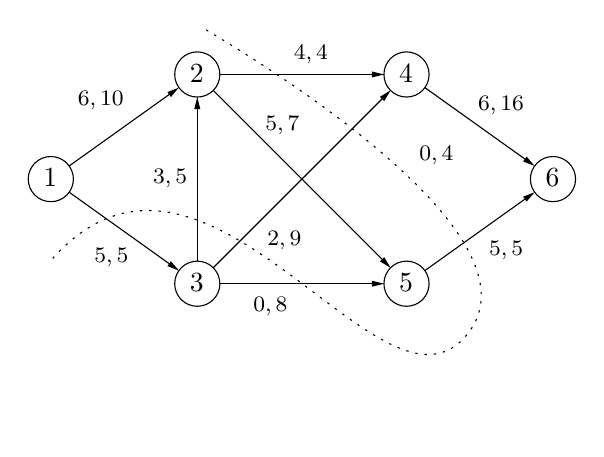
\begin{tikzpicture}[x=0.75pt,y=0.75pt,yscale=-0.8,xscale=0.8]
	%uncomment if require: \path (0,246); %set diagram left start at 0, and has height of 246

	%Curve Lines [id:da11691451855374968] 
	\draw  [dash pattern={on 0.84pt off 2.51pt}]  (61.08,153.62) .. controls (152.65,51.97) and (255.98,256.11) .. (308.07,202.35) .. controls (360.15,148.58) and (215.66,52.81) .. (151.81,15.01) ;

	% Text Node
	\draw    (59.95, 105.87) circle [x radius= 13.6, y radius= 13.6]   ;
	\draw (53.95,98.27) node [anchor=north west][inner sep=0.75pt]    {$1$};
	% Text Node
	\draw    (148.16, 42.86) circle [x radius= 13.6, y radius= 13.6]   ;
	\draw (142.16,35.26) node [anchor=north west][inner sep=0.75pt]    {$2$};
	% Text Node
	\draw    (148.16, 168.87) circle [x radius= 13.6, y radius= 13.6]   ;
	\draw (142.16,161.27) node [anchor=north west][inner sep=0.75pt]    {$3$};
	% Text Node
	\draw    (274.17, 42.86) circle [x radius= 13.6, y radius= 13.6]   ;
	\draw (268.17,35.26) node [anchor=north west][inner sep=0.75pt]    {$4$};
	% Text Node
	\draw    (274.17, 168.87) circle [x radius= 13.6, y radius= 13.6]   ;
	\draw (268.17,161.27) node [anchor=north west][inner sep=0.75pt]    {$5$};
	% Text Node
	\draw    (362.38, 105.87) circle [x radius= 13.6, y radius= 13.6]   ;
	\draw (356.38,98.27) node [anchor=north west][inner sep=0.75pt]    {$6$};
	% Text Node
	\draw (74.64,51.12) node [anchor=north west][inner sep=0.75pt]  [font=\footnotesize]  {$6,10$};
	% Text Node
	\draw (204.79,23.4) node [anchor=north west][inner sep=0.75pt]  [font=\footnotesize]  {$4,4$};
	% Text Node
	\draw (315.75,54.48) node [anchor=north west][inner sep=0.75pt]  [font=\footnotesize]  {$6,16$};
	% Text Node
	\draw (322.4,141.85) node [anchor=north west][inner sep=0.75pt]  [font=\footnotesize]  {$5,5$};
	% Text Node
	\draw (280.39,84.73) node [anchor=north west][inner sep=0.75pt]  [font=\footnotesize]  {$0,4$};
	% Text Node
	\draw (187.57,66.24) node [anchor=north west][inner sep=0.75pt]  [font=\footnotesize]  {$5,7$};
	% Text Node
	\draw (188.83,135.97) node [anchor=north west][inner sep=0.75pt]  [font=\footnotesize]  {$2,9$};
	% Text Node
	\draw (119.94,98.17) node [anchor=north west][inner sep=0.75pt]  [font=\footnotesize]  {$3,5$};
	% Text Node
	\draw (180.42,175.46) node [anchor=north west][inner sep=0.75pt]  [font=\footnotesize]  {$0,8$};
	% Text Node
	\draw (84.65,146.05) node [anchor=north west][inner sep=0.75pt]  [font=\footnotesize]  {$5,5$};
	% Connection
	\draw    (71.02,97.96) -- (135.46,51.93) ;
	\draw [shift={(137.09,50.77)}, rotate = 144.46] [fill={rgb, 255:red, 0; green, 0; blue, 0 }  ][line width=0.08]  [draw opacity=0] (7.2,-1.8) -- (0,0) -- (7.2,1.8) -- cycle    ;
	% Connection
	\draw    (71.02,113.77) -- (135.46,159.81) ;
	\draw [shift={(137.09,160.97)}, rotate = 215.54] [fill={rgb, 255:red, 0; green, 0; blue, 0 }  ][line width=0.08]  [draw opacity=0] (7.2,-1.8) -- (0,0) -- (7.2,1.8) -- cycle    ;
	% Connection
	\draw    (148.16,155.27) -- (148.16,58.46) ;
	\draw [shift={(148.16,56.46)}, rotate = 90] [fill={rgb, 255:red, 0; green, 0; blue, 0 }  ][line width=0.08]  [draw opacity=0] (7.2,-1.8) -- (0,0) -- (7.2,1.8) -- cycle    ;
	% Connection
	\draw    (157.78,159.26) -- (263.14,53.89) ;
	\draw [shift={(264.56,52.48)}, rotate = 135] [fill={rgb, 255:red, 0; green, 0; blue, 0 }  ][line width=0.08]  [draw opacity=0] (7.2,-1.8) -- (0,0) -- (7.2,1.8) -- cycle    ;
	% Connection
	\draw    (161.76,168.87) -- (258.57,168.87) ;
	\draw [shift={(260.57,168.87)}, rotate = 180] [fill={rgb, 255:red, 0; green, 0; blue, 0 }  ][line width=0.08]  [draw opacity=0] (7.2,-1.8) -- (0,0) -- (7.2,1.8) -- cycle    ;
	% Connection
	\draw    (161.76,42.86) -- (258.57,42.86) ;
	\draw [shift={(260.57,42.86)}, rotate = 180] [fill={rgb, 255:red, 0; green, 0; blue, 0 }  ][line width=0.08]  [draw opacity=0] (7.2,-1.8) -- (0,0) -- (7.2,1.8) -- cycle    ;
	% Connection
	\draw    (157.78,52.48) -- (263.14,157.84) ;
	\draw [shift={(264.56,159.26)}, rotate = 225] [fill={rgb, 255:red, 0; green, 0; blue, 0 }  ][line width=0.08]  [draw opacity=0] (7.2,-1.8) -- (0,0) -- (7.2,1.8) -- cycle    ;
	% Connection
	\draw    (285.24,160.97) -- (349.69,114.94) ;
	\draw [shift={(351.31,113.77)}, rotate = 144.46] [fill={rgb, 255:red, 0; green, 0; blue, 0 }  ][line width=0.08]  [draw opacity=0] (7.2,-1.8) -- (0,0) -- (7.2,1.8) -- cycle    ;
	% Connection
	\draw    (285.24,50.77) -- (349.69,96.8) ;
	\draw [shift={(351.31,97.96)}, rotate = 215.54] [fill={rgb, 255:red, 0; green, 0; blue, 0 }  ][line width=0.08]  [draw opacity=0] (7.2,-1.8) -- (0,0) -- (7.2,1.8) -- cycle    ;

	\end{tikzpicture}
\end{figure}
\FloatBarrier

$s=1,t=6$.

$N_{s} =\{1,2,5\} ,N_{t} =\{3,4,6\}$.

\begin{figure}[htpb]
	\centering
	\tikzset{every picture/.style={line width=0.75pt}} %set default line width to 0.75pt        

	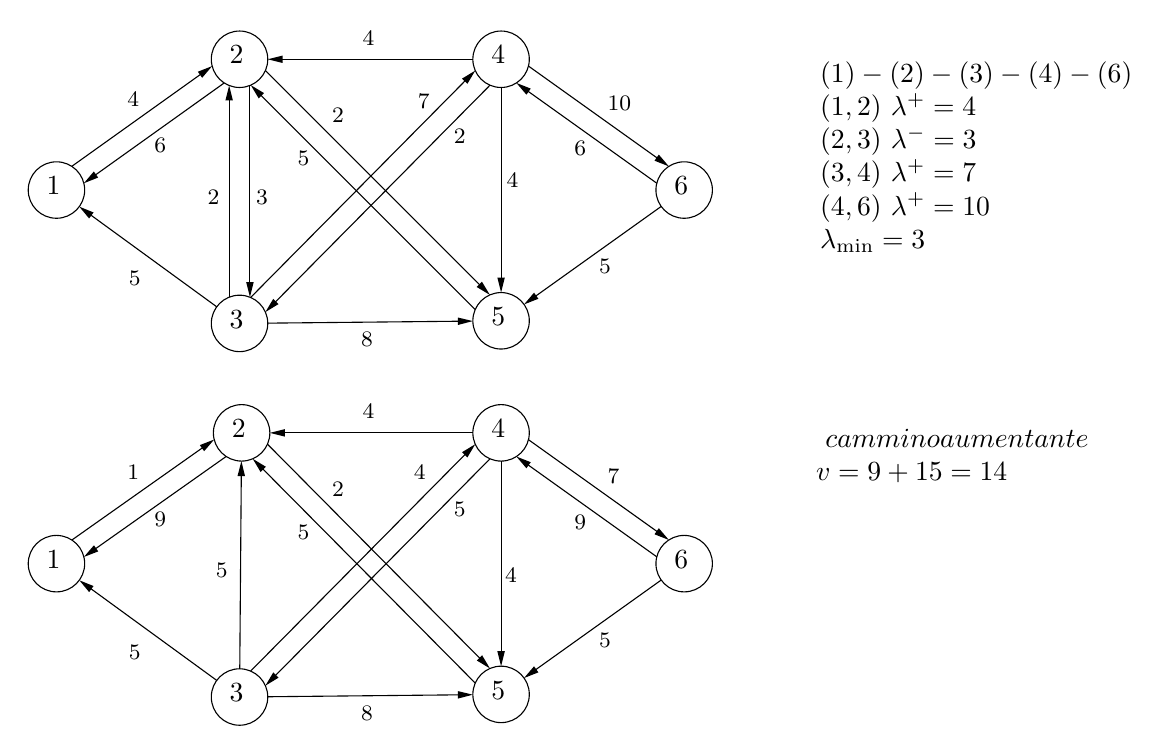
\begin{tikzpicture}[x=0.75pt,y=0.75pt,yscale=-1,xscale=1]
	%uncomment if require: \path (0,379); %set diagram left start at 0, and has height of 379


	% Text Node
	\draw    (39.95, 98.49) circle [x radius= 13.6, y radius= 13.6]   ;
	\draw (33.95,90.89) node [anchor=north west][inner sep=0.75pt]    {$1$};
	% Text Node
	\draw    (128.16, 35.48) circle [x radius= 13.6, y radius= 13.6]   ;
	\draw (122.16,27.88) node [anchor=north west][inner sep=0.75pt]    {$2$};
	% Text Node
	\draw    (128.16, 162.75) circle [x radius= 13.6, y radius= 13.6]   ;
	\draw (122.16,155.15) node [anchor=north west][inner sep=0.75pt]    {$3$};
	% Text Node
	\draw    (254.17, 35.48) circle [x radius= 13.6, y radius= 13.6]   ;
	\draw (248.17,27.88) node [anchor=north west][inner sep=0.75pt]    {$4$};
	% Text Node
	\draw    (254.17, 161.49) circle [x radius= 13.6, y radius= 13.6]   ;
	\draw (248.17,153.89) node [anchor=north west][inner sep=0.75pt]    {$5$};
	% Text Node
	\draw    (342.38, 98.49) circle [x radius= 13.6, y radius= 13.6]   ;
	\draw (336.38,90.89) node [anchor=north west][inner sep=0.75pt]    {$6$};
	% Text Node
	\draw (85.87,72.44) node [anchor=north west][inner sep=0.75pt]  [font=\footnotesize]  {$6$};
	% Text Node
	\draw (72.85,49.87) node [anchor=north west][inner sep=0.75pt]  [font=\footnotesize]  {$4$};
	% Text Node
	\draw (73.52,136.53) node [anchor=north west][inner sep=0.75pt]  [font=\footnotesize]  {$5$};
	% Text Node
	\draw (154.85,78.53) node [anchor=north west][inner sep=0.75pt]  [font=\footnotesize]  {$5$};
	% Text Node
	\draw (171.52,57.87) node [anchor=north west][inner sep=0.75pt]  [font=\footnotesize]  {$2$};
	% Text Node
	\draw (186.18,20.53) node [anchor=north west][inner sep=0.75pt]  [font=\footnotesize]  {$4$};
	% Text Node
	\draw (111.52,97.2) node [anchor=north west][inner sep=0.75pt]  [font=\footnotesize]  {$2$};
	% Text Node
	\draw (134.85,97.2) node [anchor=north west][inner sep=0.75pt]  [font=\footnotesize]  {$3$};
	% Text Node
	\draw (230.18,67.87) node [anchor=north west][inner sep=0.75pt]  [font=\footnotesize]  {$2$};
	% Text Node
	\draw (212.85,51.2) node [anchor=north west][inner sep=0.75pt]  [font=\footnotesize]  {$7$};
	% Text Node
	\draw (304.18,51.87) node [anchor=north west][inner sep=0.75pt]  [font=\footnotesize]  {$10$};
	% Text Node
	\draw (288.18,73.87) node [anchor=north west][inner sep=0.75pt]  [font=\footnotesize]  {$6$};
	% Text Node
	\draw (300.18,130.53) node [anchor=north west][inner sep=0.75pt]  [font=\footnotesize]  {$5$};
	% Text Node
	\draw (185.52,165.87) node [anchor=north west][inner sep=0.75pt]  [font=\footnotesize]  {$8$};
	% Text Node
	\draw (400,34.07) node [anchor=north west][inner sep=0.75pt]    {$ \begin{array}{l}
	( 1) -( 2) -( 3) -( 4) -( 6)\\
	( 1,2) \ \lambda ^{+} =4\\
	( 2,3) \ \lambda ^{-} =3\\
	( 3,4) \ \lambda ^{+} =7\\
	( 4,6) \ \lambda ^{+} =10\\
	\lambda _{\min} =3
	\end{array}$};
	% Text Node
	\draw    (39.95, 278.49) circle [x radius= 13.6, y radius= 13.6]   ;
	\draw (33.95,270.89) node [anchor=north west][inner sep=0.75pt]    {$1$};
	% Text Node
	\draw    (129.16, 215.48) circle [x radius= 13.6, y radius= 13.6]   ;
	\draw (123.16,207.88) node [anchor=north west][inner sep=0.75pt]    {$2$};
	% Text Node
	\draw    (128.16, 342.75) circle [x radius= 13.6, y radius= 13.6]   ;
	\draw (122.16,335.15) node [anchor=north west][inner sep=0.75pt]    {$3$};
	% Text Node
	\draw    (254.17, 215.48) circle [x radius= 13.6, y radius= 13.6]   ;
	\draw (248.17,207.88) node [anchor=north west][inner sep=0.75pt]    {$4$};
	% Text Node
	\draw    (254.17, 341.49) circle [x radius= 13.6, y radius= 13.6]   ;
	\draw (248.17,333.89) node [anchor=north west][inner sep=0.75pt]    {$5$};
	% Text Node
	\draw    (342.38, 278.49) circle [x radius= 13.6, y radius= 13.6]   ;
	\draw (336.38,270.89) node [anchor=north west][inner sep=0.75pt]    {$6$};
	% Text Node
	\draw (85.87,252.44) node [anchor=north west][inner sep=0.75pt]  [font=\footnotesize]  {$9$};
	% Text Node
	\draw (72.85,229.87) node [anchor=north west][inner sep=0.75pt]  [font=\footnotesize]  {$1$};
	% Text Node
	\draw (73.52,316.53) node [anchor=north west][inner sep=0.75pt]  [font=\footnotesize]  {$5$};
	% Text Node
	\draw (154.85,258.53) node [anchor=north west][inner sep=0.75pt]  [font=\footnotesize]  {$5$};
	% Text Node
	\draw (171.52,237.87) node [anchor=north west][inner sep=0.75pt]  [font=\footnotesize]  {$2$};
	% Text Node
	\draw (186.18,200.53) node [anchor=north west][inner sep=0.75pt]  [font=\footnotesize]  {$4$};
	% Text Node
	\draw (115.52,277.2) node [anchor=north west][inner sep=0.75pt]  [font=\footnotesize]  {$5$};
	% Text Node
	\draw (230.18,247.87) node [anchor=north west][inner sep=0.75pt]  [font=\footnotesize]  {$5$};
	% Text Node
	\draw (210.85,229.87) node [anchor=north west][inner sep=0.75pt]  [font=\footnotesize]  {$4$};
	% Text Node
	\draw (304.18,231.87) node [anchor=north west][inner sep=0.75pt]  [font=\footnotesize]  {$7$};
	% Text Node
	\draw (288.18,253.87) node [anchor=north west][inner sep=0.75pt]  [font=\footnotesize]  {$9$};
	% Text Node
	\draw (300.18,310.53) node [anchor=north west][inner sep=0.75pt]  [font=\footnotesize]  {$5$};
	% Text Node
	\draw (185.52,345.87) node [anchor=north west][inner sep=0.75pt]  [font=\footnotesize]  {$8$};
	% Text Node
	\draw (255.52,89.2) node [anchor=north west][inner sep=0.75pt]  [font=\footnotesize]  {$4$};
	% Text Node
	\draw (254.85,279.2) node [anchor=north west][inner sep=0.75pt]  [font=\footnotesize]  {$4$};
	% Text Node
	\draw (398,210.07) node [anchor=north west][inner sep=0.75pt]    {$ \begin{array}{l}
	\nexists \ \text{cammino aumentante}\\
	v=9+15=14
	\end{array}$};
	% Connection
	\draw    (47.34,87.07) -- (113.33,39.93) ;
	\draw [shift={(114.96,38.77)}, rotate = 144.46] [fill={rgb, 255:red, 0; green, 0; blue, 0 }  ][line width=0.08]  [draw opacity=0] (7.2,-1.8) -- (0,0) -- (7.2,1.8) -- cycle    ;
	% Connection
	\draw    (123.16,150.1) -- (123.16,50.13) ;
	\draw [shift={(123.16,48.13)}, rotate = 90] [fill={rgb, 255:red, 0; green, 0; blue, 0 }  ][line width=0.08]  [draw opacity=0] (7.2,-1.8) -- (0,0) -- (7.2,1.8) -- cycle    ;
	% Connection
	\draw    (133.51,150.24) -- (240.31,42.37) ;
	\draw [shift={(241.72,40.95)}, rotate = 134.71] [fill={rgb, 255:red, 0; green, 0; blue, 0 }  ][line width=0.08]  [draw opacity=0] (7.2,-1.8) -- (0,0) -- (7.2,1.8) -- cycle    ;
	% Connection
	\draw    (141.76,162.62) -- (238.57,161.65) ;
	\draw [shift={(240.57,161.63)}, rotate = 179.43] [fill={rgb, 255:red, 0; green, 0; blue, 0 }  ][line width=0.08]  [draw opacity=0] (7.2,-1.8) -- (0,0) -- (7.2,1.8) -- cycle    ;
	% Connection
	\draw    (140.64,40.89) -- (247.35,147.6) ;
	\draw [shift={(248.76,149.01)}, rotate = 225] [fill={rgb, 255:red, 0; green, 0; blue, 0 }  ][line width=0.08]  [draw opacity=0] (7.2,-1.8) -- (0,0) -- (7.2,1.8) -- cycle    ;
	% Connection
	\draw    (254.17,49.08) -- (254.17,145.89) ;
	\draw [shift={(254.17,147.89)}, rotate = 270] [fill={rgb, 255:red, 0; green, 0; blue, 0 }  ][line width=0.08]  [draw opacity=0] (7.2,-1.8) -- (0,0) -- (7.2,1.8) -- cycle    ;
	% Connection
	\draw    (267.38,38.77) -- (333.37,85.9) ;
	\draw [shift={(334.99,87.07)}, rotate = 215.54] [fill={rgb, 255:red, 0; green, 0; blue, 0 }  ][line width=0.08]  [draw opacity=0] (7.2,-1.8) -- (0,0) -- (7.2,1.8) -- cycle    ;
	% Connection
	\draw    (120.77,46.9) -- (54.78,94.04) ;
	\draw [shift={(53.15,95.2)}, rotate = 324.46] [fill={rgb, 255:red, 0; green, 0; blue, 0 }  ][line width=0.08]  [draw opacity=0] (7.2,-1.8) -- (0,0) -- (7.2,1.8) -- cycle    ;
	% Connection
	\draw    (117.17,154.74) -- (52.56,107.67) ;
	\draw [shift={(50.94,106.5)}, rotate = 36.08] [fill={rgb, 255:red, 0; green, 0; blue, 0 }  ][line width=0.08]  [draw opacity=0] (7.2,-1.8) -- (0,0) -- (7.2,1.8) -- cycle    ;
	% Connection
	\draw    (133.16,48.13) -- (133.16,148.1) ;
	\draw [shift={(133.16,150.1)}, rotate = 270] [fill={rgb, 255:red, 0; green, 0; blue, 0 }  ][line width=0.08]  [draw opacity=0] (7.2,-1.8) -- (0,0) -- (7.2,1.8) -- cycle    ;
	% Connection
	\draw    (248.82,47.99) -- (142.02,155.86) ;
	\draw [shift={(140.62,157.28)}, rotate = 314.71] [fill={rgb, 255:red, 0; green, 0; blue, 0 }  ][line width=0.08]  [draw opacity=0] (7.2,-1.8) -- (0,0) -- (7.2,1.8) -- cycle    ;
	% Connection
	\draw    (240.57,35.48) -- (143.76,35.48) ;
	\draw [shift={(141.76,35.48)}, rotate = 360] [fill={rgb, 255:red, 0; green, 0; blue, 0 }  ][line width=0.08]  [draw opacity=0] (7.2,-1.8) -- (0,0) -- (7.2,1.8) -- cycle    ;
	% Connection
	\draw    (329.18,95.2) -- (263.19,48.06) ;
	\draw [shift={(261.56,46.9)}, rotate = 35.54] [fill={rgb, 255:red, 0; green, 0; blue, 0 }  ][line width=0.08]  [draw opacity=0] (7.2,-1.8) -- (0,0) -- (7.2,1.8) -- cycle    ;
	% Connection
	\draw    (331.31,106.39) -- (266.87,152.42) ;
	\draw [shift={(265.24,153.59)}, rotate = 324.46] [fill={rgb, 255:red, 0; green, 0; blue, 0 }  ][line width=0.08]  [draw opacity=0] (7.2,-1.8) -- (0,0) -- (7.2,1.8) -- cycle    ;
	% Connection
	\draw    (241.69,156.08) -- (134.99,49.38) ;
	\draw [shift={(133.57,47.96)}, rotate = 45] [fill={rgb, 255:red, 0; green, 0; blue, 0 }  ][line width=0.08]  [draw opacity=0] (7.2,-1.8) -- (0,0) -- (7.2,1.8) -- cycle    ;
	% Connection
	\draw    (47.4,267.1) -- (114.31,219.85) ;
	\draw [shift={(115.94,218.7)}, rotate = 144.77] [fill={rgb, 255:red, 0; green, 0; blue, 0 }  ][line width=0.08]  [draw opacity=0] (7.2,-1.8) -- (0,0) -- (7.2,1.8) -- cycle    ;
	% Connection
	\draw    (128.27,329.15) -- (129.04,231.08) ;
	\draw [shift={(129.05,229.08)}, rotate = 90.45] [fill={rgb, 255:red, 0; green, 0; blue, 0 }  ][line width=0.08]  [draw opacity=0] (7.2,-1.8) -- (0,0) -- (7.2,1.8) -- cycle    ;
	% Connection
	\draw    (133.51,330.24) -- (240.31,222.37) ;
	\draw [shift={(241.72,220.95)}, rotate = 134.71] [fill={rgb, 255:red, 0; green, 0; blue, 0 }  ][line width=0.08]  [draw opacity=0] (7.2,-1.8) -- (0,0) -- (7.2,1.8) -- cycle    ;
	% Connection
	\draw    (141.76,342.62) -- (238.57,341.65) ;
	\draw [shift={(240.57,341.63)}, rotate = 179.43] [fill={rgb, 255:red, 0; green, 0; blue, 0 }  ][line width=0.08]  [draw opacity=0] (7.2,-1.8) -- (0,0) -- (7.2,1.8) -- cycle    ;
	% Connection
	\draw    (141.62,220.94) -- (247.4,327.57) ;
	\draw [shift={(248.81,328.99)}, rotate = 225.23] [fill={rgb, 255:red, 0; green, 0; blue, 0 }  ][line width=0.08]  [draw opacity=0] (7.2,-1.8) -- (0,0) -- (7.2,1.8) -- cycle    ;
	% Connection
	\draw    (254.17,229.08) -- (254.17,325.89) ;
	\draw [shift={(254.17,327.89)}, rotate = 270] [fill={rgb, 255:red, 0; green, 0; blue, 0 }  ][line width=0.08]  [draw opacity=0] (7.2,-1.8) -- (0,0) -- (7.2,1.8) -- cycle    ;
	% Connection
	\draw    (267.38,218.77) -- (333.37,265.9) ;
	\draw [shift={(334.99,267.07)}, rotate = 215.54] [fill={rgb, 255:red, 0; green, 0; blue, 0 }  ][line width=0.08]  [draw opacity=0] (7.2,-1.8) -- (0,0) -- (7.2,1.8) -- cycle    ;
	% Connection
	\draw    (121.71,226.86) -- (54.8,274.12) ;
	\draw [shift={(53.17,275.27)}, rotate = 324.77] [fill={rgb, 255:red, 0; green, 0; blue, 0 }  ][line width=0.08]  [draw opacity=0] (7.2,-1.8) -- (0,0) -- (7.2,1.8) -- cycle    ;
	% Connection
	\draw    (117.17,334.74) -- (52.56,287.67) ;
	\draw [shift={(50.94,286.5)}, rotate = 36.08] [fill={rgb, 255:red, 0; green, 0; blue, 0 }  ][line width=0.08]  [draw opacity=0] (7.2,-1.8) -- (0,0) -- (7.2,1.8) -- cycle    ;
	% Connection
	\draw    (248.82,227.99) -- (142.02,335.86) ;
	\draw [shift={(140.62,337.28)}, rotate = 314.71] [fill={rgb, 255:red, 0; green, 0; blue, 0 }  ][line width=0.08]  [draw opacity=0] (7.2,-1.8) -- (0,0) -- (7.2,1.8) -- cycle    ;
	% Connection
	\draw    (240.57,215.48) -- (144.76,215.48) ;
	\draw [shift={(142.76,215.48)}, rotate = 360] [fill={rgb, 255:red, 0; green, 0; blue, 0 }  ][line width=0.08]  [draw opacity=0] (7.2,-1.8) -- (0,0) -- (7.2,1.8) -- cycle    ;
	% Connection
	\draw    (329.18,275.2) -- (263.19,228.06) ;
	\draw [shift={(261.56,226.9)}, rotate = 35.54] [fill={rgb, 255:red, 0; green, 0; blue, 0 }  ][line width=0.08]  [draw opacity=0] (7.2,-1.8) -- (0,0) -- (7.2,1.8) -- cycle    ;
	% Connection
	\draw    (331.31,286.39) -- (266.87,332.42) ;
	\draw [shift={(265.24,333.59)}, rotate = 324.46] [fill={rgb, 255:red, 0; green, 0; blue, 0 }  ][line width=0.08]  [draw opacity=0] (7.2,-1.8) -- (0,0) -- (7.2,1.8) -- cycle    ;
	% Connection
	\draw    (241.71,336.03) -- (135.93,229.4) ;
	\draw [shift={(134.52,227.98)}, rotate = 45.23] [fill={rgb, 255:red, 0; green, 0; blue, 0 }  ][line width=0.08]  [draw opacity=0] (7.2,-1.8) -- (0,0) -- (7.2,1.8) -- cycle    ;

	\end{tikzpicture}
\end{figure}
\FloatBarrier

\Es

\begin{figure}[htpb]
	\centering


	\tikzset{every picture/.style={line width=0.75pt}} %set default line width to 0.75pt        

	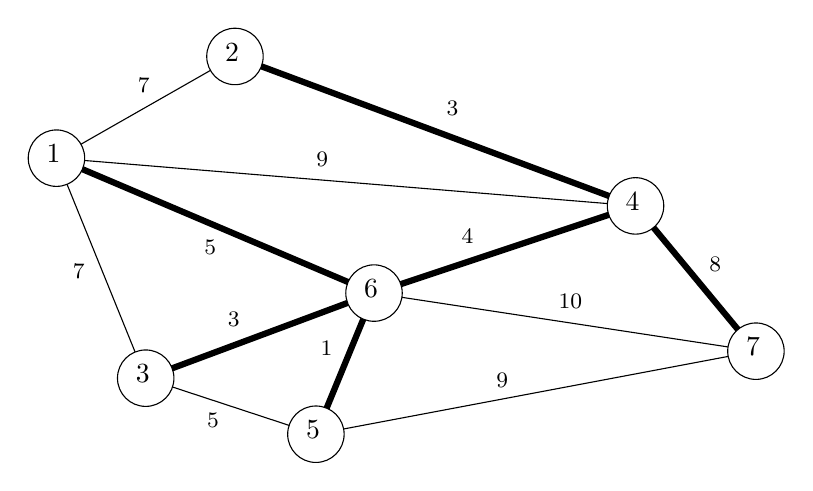
\begin{tikzpicture}[x=0.75pt,y=0.75pt,yscale=-1,xscale=1]
	%uncomment if require: \path (0,238); %set diagram left start at 0, and has height of 238


	% Text Node
	\draw    (38, 77) circle [x radius= 13.6, y radius= 13.6]   ;
	\draw (32,69.4) node [anchor=north west][inner sep=0.75pt]    {$1$};
	% Text Node
	\draw    (124, 28) circle [x radius= 13.6, y radius= 13.6]   ;
	\draw (118,20.4) node [anchor=north west][inner sep=0.75pt]    {$2$};
	% Text Node
	\draw    (81, 183) circle [x radius= 13.6, y radius= 13.6]   ;
	\draw (75,175.4) node [anchor=north west][inner sep=0.75pt]    {$3$};
	% Text Node
	\draw    (317, 100) circle [x radius= 13.6, y radius= 13.6]   ;
	\draw (311,92.4) node [anchor=north west][inner sep=0.75pt]    {$4$};
	% Text Node
	\draw    (163, 210) circle [x radius= 13.6, y radius= 13.6]   ;
	\draw (157,202.4) node [anchor=north west][inner sep=0.75pt]    {$5$};
	% Text Node
	\draw    (191, 142) circle [x radius= 13.6, y radius= 13.6]   ;
	\draw (185,134.4) node [anchor=north west][inner sep=0.75pt]    {$6$};
	% Text Node
	\draw    (375, 170) circle [x radius= 13.6, y radius= 13.6]   ;
	\draw (369,162.4) node [anchor=north west][inner sep=0.75pt]    {$7$};
	% Text Node
	\draw (76,37.4) node [anchor=north west][inner sep=0.75pt]  [font=\footnotesize]  {$7$};
	% Text Node
	\draw (224.67,48.07) node [anchor=north west][inner sep=0.75pt]  [font=\footnotesize]  {$3$};
	% Text Node
	\draw (162,72.73) node [anchor=north west][inner sep=0.75pt]  [font=\footnotesize]  {$9$};
	% Text Node
	\draw (109.33,198.73) node [anchor=north west][inner sep=0.75pt]  [font=\footnotesize]  {$5$};
	% Text Node
	\draw (44.67,126.73) node [anchor=north west][inner sep=0.75pt]  [font=\footnotesize]  {$7$};
	% Text Node
	\draw (108,115.4) node [anchor=north west][inner sep=0.75pt]  [font=\footnotesize]  {$5$};
	% Text Node
	\draw (119.33,150.07) node [anchor=north west][inner sep=0.75pt]  [font=\footnotesize]  {$3$};
	% Text Node
	\draw (164,164.07) node [anchor=north west][inner sep=0.75pt]  [font=\footnotesize]  {$1$};
	% Text Node
	\draw (232,110.07) node [anchor=north west][inner sep=0.75pt]  [font=\footnotesize]  {$4$};
	% Text Node
	\draw (278.67,141.4) node [anchor=north west][inner sep=0.75pt]  [font=\footnotesize]  {$10$};
	% Text Node
	\draw (248.67,179.4) node [anchor=north west][inner sep=0.75pt]  [font=\footnotesize]  {$9$};
	% Text Node
	\draw (351.33,123.4) node [anchor=north west][inner sep=0.75pt]  [font=\footnotesize]  {$8$};
	% Connection
	\draw    (43.11,89.61) -- (75.89,170.39) ;
	% Connection
	\draw [line width=2.25]    (93.75,178.25) -- (178.25,146.75) ;
	% Connection
	\draw    (93.92,187.26) -- (150.08,205.74) ;
	% Connection
	\draw    (112.18,34.73) -- (49.82,70.27) ;
	% Connection
	\draw [line width=2.25]    (136.75,32.76) -- (304.25,95.24) ;
	% Connection
	\draw    (51.56,78.12) -- (303.44,98.88) ;
	% Connection
	\draw [line width=2.25]    (50.52,82.32) -- (178.48,136.68) ;
	% Connection
	\draw [line width=2.25]    (203.91,137.7) -- (304.09,104.3) ;
	% Connection
	\draw [line width=2.25]    (185.82,154.58) -- (168.18,197.42) ;
	% Connection
	\draw    (204.45,144.05) -- (361.55,167.95) ;
	% Connection
	\draw [line width=2.25]    (366.32,159.53) -- (325.68,110.47) ;
	% Connection
	\draw    (361.63,172.52) -- (176.37,207.48) ;

	\end{tikzpicture}
\end{figure}
\FloatBarrier

\begin{equation*}
\begin{array}{ c c c c }
\text{Lato} & \text{Costo} & \text{Accettato} & | T| \\
( 5,6) & 1 & \text{\cmark}  & 1\\
( 3,6) & 3 & \text{\cmark}  & 2\\
( 2,4) & 3 & \text{\cmark}  & 3\\
( 4,6) & 4 & \text{\cmark}  & 4\\
( 1,6) & 5 & \text{\cmark}  & 5\\
( 3,5) & 5 & \text{\xmark}  & \\
( 1,2) & 7 & \text{\xmark}  & \\
( 1,3) & 7 & \text{\xmark}  & \\
( 4,7) & 8 & \text{\cmark}  & 6\\
( 5,7) & 9 &  & \\
( 1,4) & 9 &  & \\
( 6,7) & 10 &  & 
\end{array}
\end{equation*}
\Es

\begin{figure}[htpb]
	\centering
	\tikzset{every picture/.style={line width=0.75pt}} %set default line width to 0.75pt        

	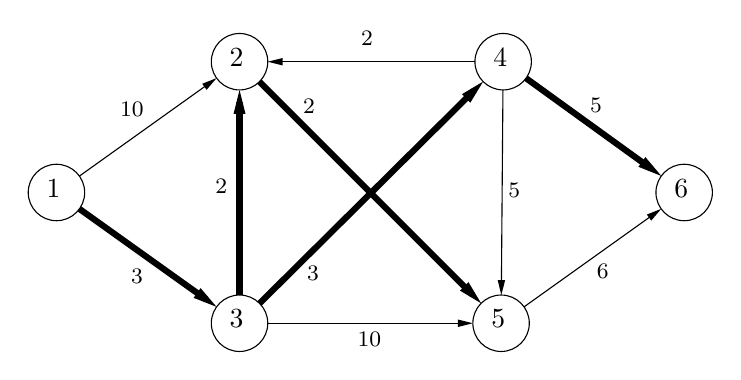
\begin{tikzpicture}[x=0.75pt,y=0.75pt,yscale=-1,xscale=1]
	%uncomment if require: \path (0,197); %set diagram left start at 0, and has height of 197


	% Text Node
	\draw    (39.95, 95.87) circle [x radius= 13.6, y radius= 13.6]   ;
	\draw (33.95,88.27) node [anchor=north west][inner sep=0.75pt]    {$1$};
	% Text Node
	\draw    (128.16, 32.86) circle [x radius= 13.6, y radius= 13.6]   ;
	\draw (122.16,25.26) node [anchor=north west][inner sep=0.75pt]    {$2$};
	% Text Node
	\draw    (128.16, 158.87) circle [x radius= 13.6, y radius= 13.6]   ;
	\draw (122.16,151.27) node [anchor=north west][inner sep=0.75pt]    {$3$};
	% Text Node
	\draw    (255.17, 32.86) circle [x radius= 13.6, y radius= 13.6]   ;
	\draw (249.17,25.26) node [anchor=north west][inner sep=0.75pt]    {$4$};
	% Text Node
	\draw    (254.17, 158.87) circle [x radius= 13.6, y radius= 13.6]   ;
	\draw (248.17,151.27) node [anchor=north west][inner sep=0.75pt]    {$5$};
	% Text Node
	\draw    (342.38, 95.87) circle [x radius= 13.6, y radius= 13.6]   ;
	\draw (336.38,88.27) node [anchor=north west][inner sep=0.75pt]    {$6$};
	% Text Node
	\draw (69.31,51.12) node [anchor=north west][inner sep=0.75pt]  [font=\footnotesize]  {$10$};
	% Text Node
	\draw (185.45,16.73) node [anchor=north west][inner sep=0.75pt]  [font=\footnotesize]  {$2$};
	% Text Node
	\draw (295.75,49.15) node [anchor=north west][inner sep=0.75pt]  [font=\footnotesize]  {$5$};
	% Text Node
	\draw (299.07,129.19) node [anchor=north west][inner sep=0.75pt]  [font=\footnotesize]  {$6$};
	% Text Node
	\draw (256.39,90.06) node [anchor=north west][inner sep=0.75pt]  [font=\footnotesize]  {$5$};
	% Text Node
	\draw (157.57,49.58) node [anchor=north west][inner sep=0.75pt]  [font=\footnotesize]  {$2$};
	% Text Node
	\draw (159.49,129.97) node [anchor=north west][inner sep=0.75pt]  [font=\footnotesize]  {$3$};
	% Text Node
	\draw (115.27,88.17) node [anchor=north west][inner sep=0.75pt]  [font=\footnotesize]  {$2$};
	% Text Node
	\draw (183.76,162.12) node [anchor=north west][inner sep=0.75pt]  [font=\footnotesize]  {$10$};
	% Text Node
	\draw (74.65,131.39) node [anchor=north west][inner sep=0.75pt]  [font=\footnotesize]  {$3$};
	% Connection
	\draw    (51.02,87.96) -- (115.46,41.93) ;
	\draw [shift={(117.09,40.77)}, rotate = 144.46] [fill={rgb, 255:red, 0; green, 0; blue, 0 }  ][line width=0.08]  [draw opacity=0] (7.2,-1.8) -- (0,0) -- (7.2,1.8) -- cycle    ;
	% Connection
	\draw [line width=2.25]    (51.02,103.77) -- (112.21,147.48) ;
	\draw [shift={(117.09,150.97)}, rotate = 215.54] [fill={rgb, 255:red, 0; green, 0; blue, 0 }  ][line width=0.08]  [draw opacity=0] (11.52,-2.88) -- (0,0) -- (11.52,2.88) -- cycle    ;
	% Connection
	\draw [line width=2.25]    (128.16,145.27) -- (128.16,52.46) ;
	\draw [shift={(128.16,46.46)}, rotate = 90] [fill={rgb, 255:red, 0; green, 0; blue, 0 }  ][line width=0.08]  [draw opacity=0] (11.52,-2.88) -- (0,0) -- (11.52,2.88) -- cycle    ;
	% Connection
	\draw [line width=2.25]    (137.82,149.29) -- (241.26,46.67) ;
	\draw [shift={(245.52,42.44)}, rotate = 135.23] [fill={rgb, 255:red, 0; green, 0; blue, 0 }  ][line width=0.08]  [draw opacity=0] (11.52,-2.88) -- (0,0) -- (11.52,2.88) -- cycle    ;
	% Connection
	\draw    (141.76,158.87) -- (238.57,158.87) ;
	\draw [shift={(240.57,158.87)}, rotate = 180] [fill={rgb, 255:red, 0; green, 0; blue, 0 }  ][line width=0.08]  [draw opacity=0] (7.2,-1.8) -- (0,0) -- (7.2,1.8) -- cycle    ;
	% Connection
	\draw [line width=2.25]    (137.78,42.48) -- (240.31,145.01) ;
	\draw [shift={(244.56,149.26)}, rotate = 225] [fill={rgb, 255:red, 0; green, 0; blue, 0 }  ][line width=0.08]  [draw opacity=0] (11.52,-2.88) -- (0,0) -- (11.52,2.88) -- cycle    ;
	% Connection
	\draw    (265.24,150.97) -- (329.69,104.94) ;
	\draw [shift={(331.31,103.77)}, rotate = 144.46] [fill={rgb, 255:red, 0; green, 0; blue, 0 }  ][line width=0.08]  [draw opacity=0] (7.2,-1.8) -- (0,0) -- (7.2,1.8) -- cycle    ;
	% Connection
	\draw [line width=2.25]    (266.2,40.83) -- (326.49,84.39) ;
	\draw [shift={(331.36,87.9)}, rotate = 215.85] [fill={rgb, 255:red, 0; green, 0; blue, 0 }  ][line width=0.08]  [draw opacity=0] (11.52,-2.88) -- (0,0) -- (11.52,2.88) -- cycle    ;
	% Connection
	\draw    (241.57,32.86) -- (143.76,32.86) ;
	\draw [shift={(141.76,32.86)}, rotate = 360] [fill={rgb, 255:red, 0; green, 0; blue, 0 }  ][line width=0.08]  [draw opacity=0] (7.2,-1.8) -- (0,0) -- (7.2,1.8) -- cycle    ;
	% Connection
	\draw    (255.07,46.46) -- (254.3,143.27) ;
	\draw [shift={(254.28,145.27)}, rotate = 270.45] [fill={rgb, 255:red, 0; green, 0; blue, 0 }  ][line width=0.08]  [draw opacity=0] (7.2,-1.8) -- (0,0) -- (7.2,1.8) -- cycle    ;

	\end{tikzpicture}
\end{figure}
\FloatBarrier

Enumerazione topologica.
\begin{equation*}
\begin{array}{ c c }
\text{Nodo} & \text{Etichetta}\\
( 1) & 1\\
( 3) & 2\\
( 4) & 3\\
( 2) & 4\\
( 5) & 5\\
( 6) & 6
\end{array}
\end{equation*}
SPT-aciclico.
\begin{equation*}
\begin{array}{ c|c|c|c|c|c|c }
\hline
i & d,P & d,P & d,P & d,P & d,P & d,P\\
\hline
1 & 0,1 &  &  &  &  & \\
2 & M,1 & 10,1 & 5,3 &  &  & \\
3 & M,1 & 3,1 &  &  &  & \\
4 & M,1 &  & 6,3 &  &  & \\
5 & M,1 &  & 13,3 & 11,4 & 7,2 & \\
6 & M,1 &  &  & 11,4 &  & \\
\hline
i & 1\ \  & 3 & 4 & 2 & 5 & 6\\
\hline
\end{array}
\end{equation*}


\Es

\begin{figure}[htpb]
	\centering
	

	\tikzset{every picture/.style={line width=0.75pt}} %set default line width to 0.75pt        

	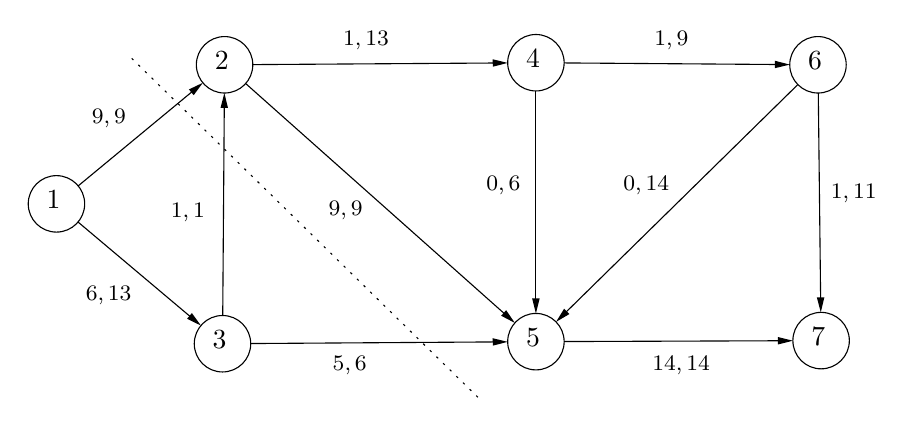
\begin{tikzpicture}[x=0.75pt,y=0.75pt,yscale=-1,xscale=1]
	%uncomment if require: \path (0,207); %set diagram left start at 0, and has height of 207

	%Straight Lines [id:da7123700015911254] 
	\draw  [dash pattern={on 0.84pt off 2.51pt}]  (77,32) -- (244,195.5) ;

	% Text Node
	\draw    (121.72, 35.09) circle [x radius= 13.6, y radius= 13.6]   ;
	\draw (115.72,27.49) node [anchor=north west][inner sep=0.75pt]    {$2$};
	% Text Node
	\draw    (120.72, 169.48) circle [x radius= 13.6, y radius= 13.6]   ;
	\draw (114.72,161.88) node [anchor=north west][inner sep=0.75pt]    {$3$};
	% Text Node
	\draw    (271.72, 34.09) circle [x radius= 13.6, y radius= 13.6]   ;
	\draw (265.72,26.49) node [anchor=north west][inner sep=0.75pt]    {$4$};
	% Text Node
	\draw    (271.72, 168.48) circle [x radius= 13.6, y radius= 13.6]   ;
	\draw (265.72,160.88) node [anchor=north west][inner sep=0.75pt]    {$5$};
	% Text Node
	\draw    (407.62, 35.09) circle [x radius= 13.6, y radius= 13.6]   ;
	\draw (401.62,27.49) node [anchor=north west][inner sep=0.75pt]    {$6$};
	% Text Node
	\draw    (409.13, 167.97) circle [x radius= 13.6, y radius= 13.6]   ;
	\draw (403.13,160.37) node [anchor=north west][inner sep=0.75pt]    {$7$};
	% Text Node
	\draw (56.57,55.47) node [anchor=north west][inner sep=0.75pt]  [font=\footnotesize]  {$9,9$};
	% Text Node
	\draw    (40.72, 102.09) circle [x radius= 13.6, y radius= 13.6]   ;
	\draw (34.72,94.49) node [anchor=north west][inner sep=0.75pt]    {$1$};
	% Text Node
	\draw (94.57,100.47) node [anchor=north west][inner sep=0.75pt]  [font=\footnotesize]  {$1,1$};
	% Text Node
	\draw (53.57,140.47) node [anchor=north west][inner sep=0.75pt]  [font=\footnotesize]  {$6,13$};
	% Text Node
	\draw (246.57,87.47) node [anchor=north west][inner sep=0.75pt]  [font=\footnotesize]  {$0,6$};
	% Text Node
	\draw (170.57,99.47) node [anchor=north west][inner sep=0.75pt]  [font=\footnotesize]  {$9,9$};
	% Text Node
	\draw (177.57,17.47) node [anchor=north west][inner sep=0.75pt]  [font=\footnotesize]  {$1,13$};
	% Text Node
	\draw (327.57,17.47) node [anchor=north west][inner sep=0.75pt]  [font=\footnotesize]  {$1,9$};
	% Text Node
	\draw (326.57,174.47) node [anchor=north west][inner sep=0.75pt]  [font=\footnotesize]  {$14,14$};
	% Text Node
	\draw (172.57,174.47) node [anchor=north west][inner sep=0.75pt]  [font=\footnotesize]  {$5,6$};
	% Text Node
	\draw (312.57,87.47) node [anchor=north west][inner sep=0.75pt]  [font=\footnotesize]  {$0,14$};
	% Text Node
	\draw (412.57,91.47) node [anchor=north west][inner sep=0.75pt]  [font=\footnotesize]  {$1,11$};
	% Connection
	\draw    (51.21,93.42) -- (109.7,45.04) ;
	\draw [shift={(111.24,43.76)}, rotate = 140.4] [fill={rgb, 255:red, 0; green, 0; blue, 0 }  ][line width=0.08]  [draw opacity=0] (7.2,-1.8) -- (0,0) -- (7.2,1.8) -- cycle    ;
	% Connection
	\draw    (51.13,110.85) -- (108.79,159.43) ;
	\draw [shift={(110.32,160.72)}, rotate = 220.11] [fill={rgb, 255:red, 0; green, 0; blue, 0 }  ][line width=0.08]  [draw opacity=0] (7.2,-1.8) -- (0,0) -- (7.2,1.8) -- cycle    ;
	% Connection
	\draw    (135.33,35) -- (256.12,34.2) ;
	\draw [shift={(258.12,34.18)}, rotate = 179.62] [fill={rgb, 255:red, 0; green, 0; blue, 0 }  ][line width=0.08]  [draw opacity=0] (7.2,-1.8) -- (0,0) -- (7.2,1.8) -- cycle    ;
	% Connection
	\draw    (131.89,44.13) -- (260.06,158.11) ;
	\draw [shift={(261.56,159.44)}, rotate = 221.65] [fill={rgb, 255:red, 0; green, 0; blue, 0 }  ][line width=0.08]  [draw opacity=0] (7.2,-1.8) -- (0,0) -- (7.2,1.8) -- cycle    ;
	% Connection
	\draw    (120.83,155.88) -- (121.61,50.69) ;
	\draw [shift={(121.62,48.69)}, rotate = 90.43] [fill={rgb, 255:red, 0; green, 0; blue, 0 }  ][line width=0.08]  [draw opacity=0] (7.2,-1.8) -- (0,0) -- (7.2,1.8) -- cycle    ;
	% Connection
	\draw    (134.33,169.39) -- (256.12,168.58) ;
	\draw [shift={(258.12,168.57)}, rotate = 179.62] [fill={rgb, 255:red, 0; green, 0; blue, 0 }  ][line width=0.08]  [draw opacity=0] (7.2,-1.8) -- (0,0) -- (7.2,1.8) -- cycle    ;
	% Connection
	\draw    (285.32,34.19) -- (392.02,34.98) ;
	\draw [shift={(394.02,34.99)}, rotate = 180.42] [fill={rgb, 255:red, 0; green, 0; blue, 0 }  ][line width=0.08]  [draw opacity=0] (7.2,-1.8) -- (0,0) -- (7.2,1.8) -- cycle    ;
	% Connection
	\draw    (271.72,47.69) -- (271.72,152.88) ;
	\draw [shift={(271.72,154.88)}, rotate = 270] [fill={rgb, 255:red, 0; green, 0; blue, 0 }  ][line width=0.08]  [draw opacity=0] (7.2,-1.8) -- (0,0) -- (7.2,1.8) -- cycle    ;
	% Connection
	\draw    (285.32,168.43) -- (393.53,168.03) ;
	\draw [shift={(395.53,168.02)}, rotate = 179.79] [fill={rgb, 255:red, 0; green, 0; blue, 0 }  ][line width=0.08]  [draw opacity=0] (7.2,-1.8) -- (0,0) -- (7.2,1.8) -- cycle    ;
	% Connection
	\draw    (397.91,44.62) -- (282.86,157.55) ;
	\draw [shift={(281.43,158.95)}, rotate = 315.53] [fill={rgb, 255:red, 0; green, 0; blue, 0 }  ][line width=0.08]  [draw opacity=0] (7.2,-1.8) -- (0,0) -- (7.2,1.8) -- cycle    ;
	% Connection
	\draw    (407.77,48.69) -- (408.95,152.37) ;
	\draw [shift={(408.97,154.37)}, rotate = 269.35] [fill={rgb, 255:red, 0; green, 0; blue, 0 }  ][line width=0.08]  [draw opacity=0] (7.2,-1.8) -- (0,0) -- (7.2,1.8) -- cycle    ;

	\end{tikzpicture}
\end{figure}
\FloatBarrier

$N_{s} =\{1,3\} ,N_{t} =\{2,4,5,6,7\} ,U( N_{s} ,N_{t}) =16=v$.

\begin{figure}[htpb]
	\centering
	\tikzset{every picture/.style={line width=0.75pt}} %set default line width to 0.75pt        

	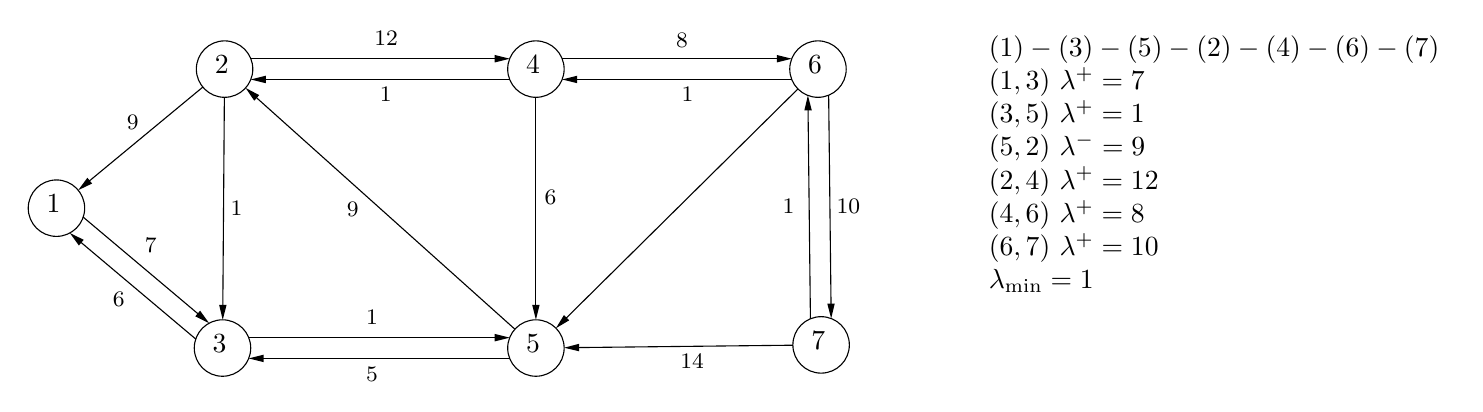
\begin{tikzpicture}[x=0.75pt,y=0.75pt,yscale=-1,xscale=1]
	%uncomment if require: \path (0,212); %set diagram left start at 0, and has height of 212


	% Text Node
	\draw    (121.72, 35.09) circle [x radius= 13.6, y radius= 13.6]   ;
	\draw (115.72,27.49) node [anchor=north west][inner sep=0.75pt]    {$2$};
	% Text Node
	\draw    (120.72, 169.48) circle [x radius= 13.6, y radius= 13.6]   ;
	\draw (114.72,161.88) node [anchor=north west][inner sep=0.75pt]    {$3$};
	% Text Node
	\draw    (271.72, 35.09) circle [x radius= 13.6, y radius= 13.6]   ;
	\draw (265.72,27.49) node [anchor=north west][inner sep=0.75pt]    {$4$};
	% Text Node
	\draw    (271.72, 169.48) circle [x radius= 13.6, y radius= 13.6]   ;
	\draw (265.72,161.88) node [anchor=north west][inner sep=0.75pt]    {$5$};
	% Text Node
	\draw    (407.62, 35.09) circle [x radius= 13.6, y radius= 13.6]   ;
	\draw (401.62,27.49) node [anchor=north west][inner sep=0.75pt]    {$6$};
	% Text Node
	\draw    (409.13, 167.97) circle [x radius= 13.6, y radius= 13.6]   ;
	\draw (403.13,160.37) node [anchor=north west][inner sep=0.75pt]    {$7$};
	% Text Node
	\draw    (40.72, 102.09) circle [x radius= 13.6, y radius= 13.6]   ;
	\draw (34.72,94.49) node [anchor=north west][inner sep=0.75pt]    {$1$};
	% Text Node
	\draw (482,16.4) node [anchor=north west][inner sep=0.75pt]    {$ \begin{array}{l}
	( 1) -( 3) -( 5) -( 2) -( 4) -( 6) -( 7)\\
	( 1,3) \ \lambda ^{+} =7\\
	( 3,5) \ \lambda ^{+} =1\\
	( 5,2) \ \lambda ^{-} =9\\
	( 2,4) \ \lambda ^{+} =12\\
	( 4,6) \ \lambda ^{+} =8\\
	( 6,7) \ \lambda ^{+} =10\\
	\lambda _{\min} =1
	\end{array}$};
	% Text Node
	\draw (73.33,56.07) node [anchor=north west][inner sep=0.75pt]  [font=\footnotesize]  {$9$};
	% Text Node
	\draw (179.33,98.07) node [anchor=north west][inner sep=0.75pt]  [font=\footnotesize]  {$9$};
	% Text Node
	\draw (192.67,15.4) node [anchor=north west][inner sep=0.75pt]  [font=\footnotesize]  {$12$};
	% Text Node
	\draw (195.33,42.73) node [anchor=north west][inner sep=0.75pt]  [font=\footnotesize]  {$1$};
	% Text Node
	\draw (340.67,42.73) node [anchor=north west][inner sep=0.75pt]  [font=\footnotesize]  {$1$};
	% Text Node
	\draw (188.67,150.07) node [anchor=north west][inner sep=0.75pt]  [font=\footnotesize]  {$1$};
	% Text Node
	\draw (389.33,96.73) node [anchor=north west][inner sep=0.75pt]  [font=\footnotesize]  {$1$};
	% Text Node
	\draw (123.33,97.4) node [anchor=north west][inner sep=0.75pt]  [font=\footnotesize]  {$1$};
	% Text Node
	\draw (82,115.4) node [anchor=north west][inner sep=0.75pt]  [font=\footnotesize]  {$7$};
	% Text Node
	\draw (66.67,141.4) node [anchor=north west][inner sep=0.75pt]  [font=\footnotesize]  {$6$};
	% Text Node
	\draw (188.67,177.4) node [anchor=north west][inner sep=0.75pt]  [font=\footnotesize]  {$5$};
	% Text Node
	\draw (340,171.4) node [anchor=north west][inner sep=0.75pt]  [font=\footnotesize]  {$14$};
	% Text Node
	\draw (415.33,96.73) node [anchor=north west][inner sep=0.75pt]  [font=\footnotesize]  {$10$};
	% Text Node
	\draw (338,16.73) node [anchor=north west][inner sep=0.75pt]  [font=\footnotesize]  {$8$};
	% Text Node
	\draw (274.67,92.07) node [anchor=north west][inner sep=0.75pt]  [font=\footnotesize]  {$6$};
	% Connection
	\draw    (53.62,106.42) -- (112.74,156.21) ;
	\draw [shift={(114.27,157.5)}, rotate = 220.11] [fill={rgb, 255:red, 0; green, 0; blue, 0 }  ][line width=0.08]  [draw opacity=0] (7.2,-1.8) -- (0,0) -- (7.2,1.8) -- cycle    ;
	% Connection
	\draw    (134.38,30.09) -- (257.07,30.09) ;
	\draw [shift={(259.07,30.09)}, rotate = 180] [fill={rgb, 255:red, 0; green, 0; blue, 0 }  ][line width=0.08]  [draw opacity=0] (7.2,-1.8) -- (0,0) -- (7.2,1.8) -- cycle    ;
	% Connection
	\draw    (133.38,164.48) -- (257.07,164.48) ;
	\draw [shift={(259.07,164.48)}, rotate = 180] [fill={rgb, 255:red, 0; green, 0; blue, 0 }  ][line width=0.08]  [draw opacity=0] (7.2,-1.8) -- (0,0) -- (7.2,1.8) -- cycle    ;
	% Connection
	\draw    (284.37,30.09) -- (392.96,30.09) ;
	\draw [shift={(394.96,30.09)}, rotate = 180] [fill={rgb, 255:red, 0; green, 0; blue, 0 }  ][line width=0.08]  [draw opacity=0] (7.2,-1.8) -- (0,0) -- (7.2,1.8) -- cycle    ;
	% Connection
	\draw    (271.72,48.69) -- (271.72,153.88) ;
	\draw [shift={(271.72,155.88)}, rotate = 270] [fill={rgb, 255:red, 0; green, 0; blue, 0 }  ][line width=0.08]  [draw opacity=0] (7.2,-1.8) -- (0,0) -- (7.2,1.8) -- cycle    ;
	% Connection
	\draw    (412.76,47.69) -- (413.96,153.26) ;
	\draw [shift={(413.98,155.26)}, rotate = 269.35] [fill={rgb, 255:red, 0; green, 0; blue, 0 }  ][line width=0.08]  [draw opacity=0] (7.2,-1.8) -- (0,0) -- (7.2,1.8) -- cycle    ;
	% Connection
	\draw    (107.83,165.15) -- (48.71,115.35) ;
	\draw [shift={(47.18,114.07)}, rotate = 40.11] [fill={rgb, 255:red, 0; green, 0; blue, 0 }  ][line width=0.08]  [draw opacity=0] (7.2,-1.8) -- (0,0) -- (7.2,1.8) -- cycle    ;
	% Connection
	\draw    (111.24,43.76) -- (52.75,92.15) ;
	\draw [shift={(51.21,93.42)}, rotate = 320.4] [fill={rgb, 255:red, 0; green, 0; blue, 0 }  ][line width=0.08]  [draw opacity=0] (7.2,-1.8) -- (0,0) -- (7.2,1.8) -- cycle    ;
	% Connection
	\draw    (259.07,40.09) -- (136.38,40.09) ;
	\draw [shift={(134.38,40.09)}, rotate = 360] [fill={rgb, 255:red, 0; green, 0; blue, 0 }  ][line width=0.08]  [draw opacity=0] (7.2,-1.8) -- (0,0) -- (7.2,1.8) -- cycle    ;
	% Connection
	\draw    (394.96,40.09) -- (286.37,40.09) ;
	\draw [shift={(284.37,40.09)}, rotate = 360] [fill={rgb, 255:red, 0; green, 0; blue, 0 }  ][line width=0.08]  [draw opacity=0] (7.2,-1.8) -- (0,0) -- (7.2,1.8) -- cycle    ;
	% Connection
	\draw    (403.98,155.37) -- (402.78,49.8) ;
	\draw [shift={(402.76,47.8)}, rotate = 89.35] [fill={rgb, 255:red, 0; green, 0; blue, 0 }  ][line width=0.08]  [draw opacity=0] (7.2,-1.8) -- (0,0) -- (7.2,1.8) -- cycle    ;
	% Connection
	\draw    (395.53,168.12) -- (287.32,169.31) ;
	\draw [shift={(285.32,169.33)}, rotate = 359.37] [fill={rgb, 255:red, 0; green, 0; blue, 0 }  ][line width=0.08]  [draw opacity=0] (7.2,-1.8) -- (0,0) -- (7.2,1.8) -- cycle    ;
	% Connection
	\draw    (397.95,44.66) -- (282.81,158.51) ;
	\draw [shift={(281.39,159.91)}, rotate = 315.32] [fill={rgb, 255:red, 0; green, 0; blue, 0 }  ][line width=0.08]  [draw opacity=0] (7.2,-1.8) -- (0,0) -- (7.2,1.8) -- cycle    ;
	% Connection
	\draw    (261.59,160.4) -- (133.34,45.5) ;
	\draw [shift={(131.85,44.17)}, rotate = 41.86] [fill={rgb, 255:red, 0; green, 0; blue, 0 }  ][line width=0.08]  [draw opacity=0] (7.2,-1.8) -- (0,0) -- (7.2,1.8) -- cycle    ;
	% Connection
	\draw    (259.07,174.48) -- (135.38,174.48) ;
	\draw [shift={(133.38,174.48)}, rotate = 360] [fill={rgb, 255:red, 0; green, 0; blue, 0 }  ][line width=0.08]  [draw opacity=0] (7.2,-1.8) -- (0,0) -- (7.2,1.8) -- cycle    ;
	% Connection
	\draw    (121.62,48.69) -- (120.84,153.88) ;
	\draw [shift={(120.83,155.88)}, rotate = 270.43] [fill={rgb, 255:red, 0; green, 0; blue, 0 }  ][line width=0.08]  [draw opacity=0] (7.2,-1.8) -- (0,0) -- (7.2,1.8) -- cycle    ;

	\end{tikzpicture}
\end{figure}
\FloatBarrier

\Es
\begin{figure}[htpb]
	\centering
	\tikzset{every picture/.style={line width=0.75pt}} %set default line width to 0.75pt        

	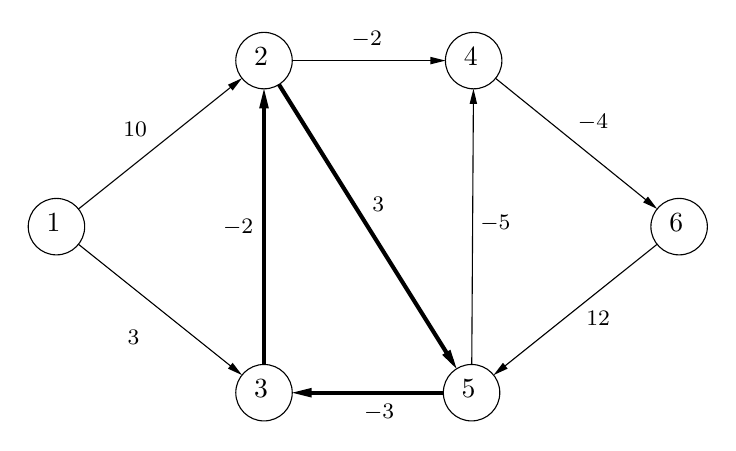
\begin{tikzpicture}[x=0.75pt,y=0.75pt,yscale=-1,xscale=1]
	%uncomment if require: \path (0,234); %set diagram left start at 0, and has height of 234


	% Text Node
	\draw    (128, 117) circle [x radius= 13.6, y radius= 13.6]   ;
	\draw (122,109.4) node [anchor=north west][inner sep=0.75pt]    {$1$};
	% Text Node
	\draw    (228, 37) circle [x radius= 13.6, y radius= 13.6]   ;
	\draw (222,29.4) node [anchor=north west][inner sep=0.75pt]    {$2$};
	% Text Node
	\draw    (228, 197) circle [x radius= 13.6, y radius= 13.6]   ;
	\draw (222,189.4) node [anchor=north west][inner sep=0.75pt]    {$3$};
	% Text Node
	\draw    (329, 37) circle [x radius= 13.6, y radius= 13.6]   ;
	\draw (323,29.4) node [anchor=north west][inner sep=0.75pt]    {$4$};
	% Text Node
	\draw    (328, 197) circle [x radius= 13.6, y radius= 13.6]   ;
	\draw (322,189.4) node [anchor=north west][inner sep=0.75pt]    {$5$};
	% Text Node
	\draw    (428, 117) circle [x radius= 13.6, y radius= 13.6]   ;
	\draw (422,109.4) node [anchor=north west][inner sep=0.75pt]    {$6$};
	% Text Node
	\draw (159,65.4) node [anchor=north west][inner sep=0.75pt]  [font=\footnotesize]  {$10$};
	% Text Node
	\draw (269,21.4) node [anchor=north west][inner sep=0.75pt]  [font=\footnotesize]  {$-2$};
	% Text Node
	\draw (207,112.4) node [anchor=north west][inner sep=0.75pt]  [font=\footnotesize]  {$-2$};
	% Text Node
	\draw (161,165.4) node [anchor=north west][inner sep=0.75pt]  [font=\footnotesize]  {$3$};
	% Text Node
	\draw (279,101.4) node [anchor=north west][inner sep=0.75pt]  [font=\footnotesize]  {$3$};
	% Text Node
	\draw (275,201.4) node [anchor=north west][inner sep=0.75pt]  [font=\footnotesize]  {$-3$};
	% Text Node
	\draw (382,156.4) node [anchor=north west][inner sep=0.75pt]  [font=\footnotesize]  {$12$};
	% Text Node
	\draw (378,61.4) node [anchor=north west][inner sep=0.75pt]  [font=\footnotesize]  {$-4$};
	% Text Node
	\draw (331,110.4) node [anchor=north west][inner sep=0.75pt]  [font=\footnotesize]  {$-5$};
	% Connection
	\draw    (138.62,125.5) -- (215.82,187.25) ;
	\draw [shift={(217.38,188.5)}, rotate = 218.66] [fill={rgb, 255:red, 0; green, 0; blue, 0 }  ][line width=0.08]  [draw opacity=0] (7.2,-1.8) -- (0,0) -- (7.2,1.8) -- cycle    ;
	% Connection
	\draw    (138.62,108.5) -- (215.82,46.75) ;
	\draw [shift={(217.38,45.5)}, rotate = 141.34] [fill={rgb, 255:red, 0; green, 0; blue, 0 }  ][line width=0.08]  [draw opacity=0] (7.2,-1.8) -- (0,0) -- (7.2,1.8) -- cycle    ;
	% Connection
	\draw [line width=1.5]    (228,183.4) -- (228,54.6) ;
	\draw [shift={(228,50.6)}, rotate = 90] [fill={rgb, 255:red, 0; green, 0; blue, 0 }  ][line width=0.08]  [draw opacity=0] (9.36,-2.34) -- (0,0) -- (9.36,2.34) -- cycle    ;
	% Connection
	\draw    (241.6,37) -- (313.4,37) ;
	\draw [shift={(315.4,37)}, rotate = 180] [fill={rgb, 255:red, 0; green, 0; blue, 0 }  ][line width=0.08]  [draw opacity=0] (7.2,-1.8) -- (0,0) -- (7.2,1.8) -- cycle    ;
	% Connection
	\draw [line width=1.5]    (235.21,48.54) -- (318.67,182.07) ;
	\draw [shift={(320.79,185.46)}, rotate = 237.99] [fill={rgb, 255:red, 0; green, 0; blue, 0 }  ][line width=0.08]  [draw opacity=0] (9.36,-2.34) -- (0,0) -- (9.36,2.34) -- cycle    ;
	% Connection
	\draw [line width=1.5]    (314.4,197) -- (245.6,197) ;
	\draw [shift={(241.6,197)}, rotate = 360] [fill={rgb, 255:red, 0; green, 0; blue, 0 }  ][line width=0.08]  [draw opacity=0] (9.36,-2.34) -- (0,0) -- (9.36,2.34) -- cycle    ;
	% Connection
	\draw    (328.09,183.4) -- (328.9,52.6) ;
	\draw [shift={(328.91,50.6)}, rotate = 90.36] [fill={rgb, 255:red, 0; green, 0; blue, 0 }  ][line width=0.08]  [draw opacity=0] (7.2,-1.8) -- (0,0) -- (7.2,1.8) -- cycle    ;
	% Connection
	\draw    (339.58,45.55) -- (415.86,107.19) ;
	\draw [shift={(417.42,108.45)}, rotate = 218.94] [fill={rgb, 255:red, 0; green, 0; blue, 0 }  ][line width=0.08]  [draw opacity=0] (7.2,-1.8) -- (0,0) -- (7.2,1.8) -- cycle    ;
	% Connection
	\draw    (417.38,125.5) -- (340.18,187.25) ;
	\draw [shift={(338.62,188.5)}, rotate = 321.34] [fill={rgb, 255:red, 0; green, 0; blue, 0 }  ][line width=0.08]  [draw opacity=0] (7.2,-1.8) -- (0,0) -- (7.2,1.8) -- cycle    ;

	\end{tikzpicture}
\end{figure}
\FloatBarrier

Cicli, costi negativi: Bellman-Ford.
\begin{equation*}
\begin{array}{ c|c|c|c|c|c|c|c|c }
\hline
i & d,P,k & d,P,k & d,P,k & d,P,k & d,P,k & d,P,k & d,P,k & d,P,k\\
\hline
1 & 0,1,1 &  &  &  &  &  &  & \\
2 & M,1,0 & 10,1,1 & 1,3,1 &  &  &  &  & -1,3,2\\
3 & M,1,0 & 3,1,1 &  &  &  &  & 1,5,2 & \\
4 & M,1,0 &  &  & -1,2,1 &  &  &  & \\
5 & M,1,0 &  &  & 4,2,1 &  &  &  & \\
6 & M,1,0 &  &  &  & -5,4,1 &  &  & \\
\hline
Q & 1 & 2,3 & 2 & 4,5 & 5,6 & 5 & 3 & 2\\
i & 1 & 3 & 2 & 4 & 6 & 5 & 3 & 2\\
\hline
\end{array}
\end{equation*}
E così via finché $k$ di $2,3$ non supera il numero soglia. Esiste un ciclo negativo
\begin{equation*}
( 2) -( 5) -( 3)
\end{equation*}

\Es

\begin{figure}[htpb]
	\centering


	\tikzset{every picture/.style={line width=0.75pt}} %set default line width to 0.75pt        

	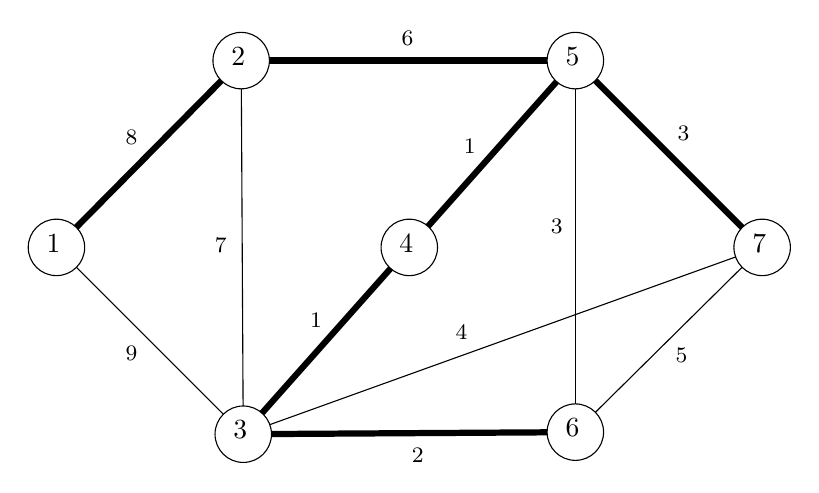
\begin{tikzpicture}[x=0.75pt,y=0.75pt,yscale=-1,xscale=1]
	%uncomment if require: \path (0,236); %set diagram left start at 0, and has height of 236


	% Text Node
	\draw    (38, 117) circle [x radius= 13.6, y radius= 13.6]   ;
	\draw (32,109.4) node [anchor=north west][inner sep=0.75pt]    {$1$};
	% Text Node
	\draw    (127, 27) circle [x radius= 13.6, y radius= 13.6]   ;
	\draw (121,19.4) node [anchor=north west][inner sep=0.75pt]    {$2$};
	% Text Node
	\draw    (128, 207) circle [x radius= 13.6, y radius= 13.6]   ;
	\draw (122,199.4) node [anchor=north west][inner sep=0.75pt]    {$3$};
	% Text Node
	\draw    (288, 27) circle [x radius= 13.6, y radius= 13.6]   ;
	\draw (282,19.4) node [anchor=north west][inner sep=0.75pt]    {$5$};
	% Text Node
	\draw    (288, 206) circle [x radius= 13.6, y radius= 13.6]   ;
	\draw (282,198.4) node [anchor=north west][inner sep=0.75pt]    {$6$};
	% Text Node
	\draw    (208, 117) circle [x radius= 13.6, y radius= 13.6]   ;
	\draw (202,109.4) node [anchor=north west][inner sep=0.75pt]    {$4$};
	% Text Node
	\draw    (378, 117) circle [x radius= 13.6, y radius= 13.6]   ;
	\draw (372,109.4) node [anchor=north west][inner sep=0.75pt]    {$7$};
	% Text Node
	\draw (70,59.4) node [anchor=north west][inner sep=0.75pt]  [font=\footnotesize]  {$8$};
	% Text Node
	\draw (113,111.4) node [anchor=north west][inner sep=0.75pt]  [font=\footnotesize]  {$7$};
	% Text Node
	\draw (70,163.4) node [anchor=north west][inner sep=0.75pt]  [font=\footnotesize]  {$9$};
	% Text Node
	\draw (203,11.4) node [anchor=north west][inner sep=0.75pt]  [font=\footnotesize]  {$6$};
	% Text Node
	\draw (336,57.4) node [anchor=north west][inner sep=0.75pt]  [font=\footnotesize]  {$3$};
	% Text Node
	\draw (275,102.4) node [anchor=north west][inner sep=0.75pt]  [font=\footnotesize]  {$3$};
	% Text Node
	\draw (208,212.4) node [anchor=north west][inner sep=0.75pt]  [font=\footnotesize]  {$2$};
	% Text Node
	\draw (159,147.4) node [anchor=north west][inner sep=0.75pt]  [font=\footnotesize]  {$1$};
	% Text Node
	\draw (233,63.4) node [anchor=north west][inner sep=0.75pt]  [font=\footnotesize]  {$1$};
	% Text Node
	\draw (229,153.4) node [anchor=north west][inner sep=0.75pt]  [font=\footnotesize]  {$4$};
	% Text Node
	\draw (335,164.4) node [anchor=north west][inner sep=0.75pt]  [font=\footnotesize]  {$5$};
	% Connection
	\draw [line width=2.25]    (47.56,107.33) -- (117.44,36.67) ;
	% Connection
	\draw    (47.62,126.62) -- (118.38,197.38) ;
	% Connection
	\draw [line width=2.25]    (141.6,206.91) -- (274.4,206.09) ;
	% Connection
	\draw    (140.8,202.39) -- (365.2,121.61) ;
	% Connection
	\draw    (127.92,193.4) -- (127.08,40.6) ;
	% Connection
	\draw [line width=2.25]    (198.96,127.17) -- (137.04,196.83) ;
	% Connection
	\draw [line width=2.25]    (217.04,106.83) -- (278.96,37.17) ;
	% Connection
	\draw [line width=2.25]    (140.6,27) -- (274.4,27) ;
	% Connection
	\draw [line width=2.25]    (297.62,36.62) -- (368.38,107.38) ;
	% Connection
	\draw    (368.33,126.56) -- (297.67,196.44) ;
	% Connection
	\draw    (288,192.4) -- (288,40.6) ;

	\end{tikzpicture}
\end{figure}
\FloatBarrier

\begin{equation*}
\begin{array}{ c c c c }
\text{Lato} & \text{Costo} & \text{Accettato} & | T| \\
( 3,4) & 1 & \text{\cmark}  & 1\\
( 4,5) & 1 & \text{\cmark}  & 2\\
( 3,6) & 2 & \text{\cmark}  & 3\\
( 5,7) & 3 & \text{\cmark}  & 4\\
( 5,6) & 3 & \text{\xmark}  & \\
( 3,7) & 4 & \text{\xmark}  & \\
( 6,7) & 5 & \text{\xmark}  & \\
( 2,5) & 6 & \text{\cmark}  & 5\\
( 3,2) & 7 & \text{\xmark}  & \\
( 1,2) & 8 & \text{\cmark}  & 6\\
( 1,3) & 9 &  & 
\end{array}
\end{equation*}
\newpage
\Es

\begin{figure}[htpb]
	\centering
	\tikzset{every picture/.style={line width=0.75pt}} %set default line width to 0.75pt        

	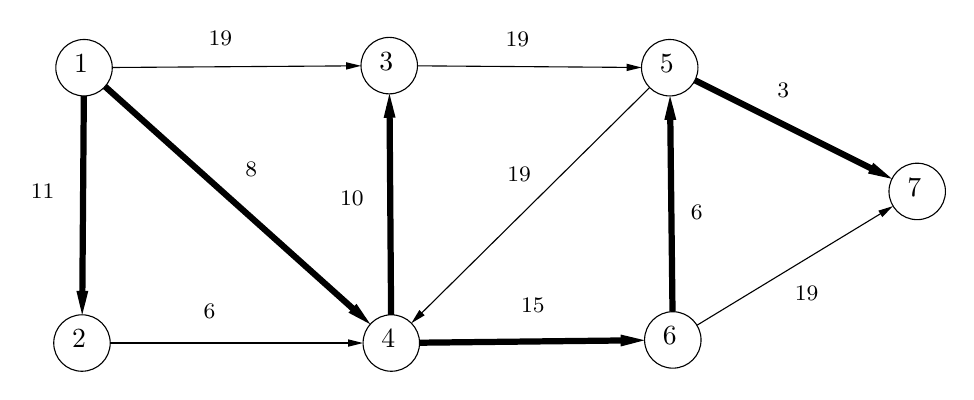
\begin{tikzpicture}[x=0.75pt,y=0.75pt,yscale=-1,xscale=1]
	%uncomment if require: \path (0,194); %set diagram left start at 0, and has height of 194


	% Text Node
	\draw    (47.3, 34.34) circle [x radius= 13.6, y radius= 13.6]   ;
	\draw (41.3,26.74) node [anchor=north west][inner sep=0.75pt]    {$1$};
	% Text Node
	\draw    (46.3, 166.99) circle [x radius= 13.6, y radius= 13.6]   ;
	\draw (40.3,159.39) node [anchor=north west][inner sep=0.75pt]    {$2$};
	% Text Node
	\draw    (194.34, 33.34) circle [x radius= 13.6, y radius= 13.6]   ;
	\draw (188.34,25.74) node [anchor=north west][inner sep=0.75pt]    {$3$};
	% Text Node
	\draw    (195.34, 166.99) circle [x radius= 13.6, y radius= 13.6]   ;
	\draw (189.34,159.39) node [anchor=north west][inner sep=0.75pt]    {$4$};
	% Text Node
	\draw    (329.48, 34.34) circle [x radius= 13.6, y radius= 13.6]   ;
	\draw (323.48,26.74) node [anchor=north west][inner sep=0.75pt]    {$5$};
	% Text Node
	\draw    (330.97, 165.5) circle [x radius= 13.6, y radius= 13.6]   ;
	\draw (324.97,157.9) node [anchor=north west][inner sep=0.75pt]    {$6$};
	% Text Node
	\draw    (448.72, 93.95) circle [x radius= 13.6, y radius= 13.6]   ;
	\draw (442.72,86.35) node [anchor=north west][inner sep=0.75pt]    {$7$};
	% Text Node
	\draw (20.41,89.1) node [anchor=north west][inner sep=0.75pt]  [font=\footnotesize]  {$11$};
	% Text Node
	\draw (169.46,92.83) node [anchor=north west][inner sep=0.75pt]  [font=\footnotesize]  {$10$};
	% Text Node
	\draw (123.76,78.67) node [anchor=north west][inner sep=0.75pt]  [font=\footnotesize]  {$8$};
	% Text Node
	\draw (103.64,147.23) node [anchor=north west][inner sep=0.75pt]  [font=\footnotesize]  {$6$};
	% Text Node
	\draw (256.65,144.25) node [anchor=north west][inner sep=0.75pt]  [font=\footnotesize]  {$15$};
	% Text Node
	\draw (249.94,80.9) node [anchor=north west][inner sep=0.75pt]  [font=\footnotesize]  {$19$};
	% Text Node
	\draw (338.39,99.53) node [anchor=north west][inner sep=0.75pt]  [font=\footnotesize]  {$6$};
	% Text Node
	\draw (388.55,138.28) node [anchor=north west][inner sep=0.75pt]  [font=\footnotesize]  {$19$};
	% Text Node
	\draw (380.12,40.66) node [anchor=north west][inner sep=0.75pt]  [font=\footnotesize]  {$3$};
	% Text Node
	\draw (249.2,16.07) node [anchor=north west][inner sep=0.75pt]  [font=\footnotesize]  {$19$};
	% Text Node
	\draw (106.11,15.32) node [anchor=north west][inner sep=0.75pt]  [font=\footnotesize]  {$19$};
	% Connection
	\draw [line width=2.25]    (47.2,47.94) -- (46.45,147.39) ;
	\draw [shift={(46.4,153.39)}, rotate = 270.43] [fill={rgb, 255:red, 0; green, 0; blue, 0 }  ][line width=0.08]  [draw opacity=0] (11.52,-2.88) -- (0,0) -- (11.52,2.88) -- cycle    ;
	% Connection
	\draw    (60.9,34.24) -- (178.74,33.44) ;
	\draw [shift={(180.74,33.43)}, rotate = 179.61] [fill={rgb, 255:red, 0; green, 0; blue, 0 }  ][line width=0.08]  [draw opacity=0] (7.2,-1.8) -- (0,0) -- (7.2,1.8) -- cycle    ;
	% Connection
	\draw [line width=2.25]    (57.43,43.41) -- (180.74,153.91) ;
	\draw [shift={(185.21,157.91)}, rotate = 221.86] [fill={rgb, 255:red, 0; green, 0; blue, 0 }  ][line width=0.08]  [draw opacity=0] (11.52,-2.88) -- (0,0) -- (11.52,2.88) -- cycle    ;
	% Connection
	\draw [line width=2.25]    (195.24,153.39) -- (194.49,52.94) ;
	\draw [shift={(194.44,46.94)}, rotate = 89.57] [fill={rgb, 255:red, 0; green, 0; blue, 0 }  ][line width=0.08]  [draw opacity=0] (11.52,-2.88) -- (0,0) -- (11.52,2.88) -- cycle    ;
	% Connection
	\draw    (59.9,166.99) -- (179.74,166.99) ;
	\draw [shift={(181.74,166.99)}, rotate = 180] [fill={rgb, 255:red, 0; green, 0; blue, 0 }  ][line width=0.08]  [draw opacity=0] (7.2,-1.8) -- (0,0) -- (7.2,1.8) -- cycle    ;
	% Connection
	\draw [line width=2.25]    (208.94,166.84) -- (311.37,165.71) ;
	\draw [shift={(317.37,165.65)}, rotate = 179.37] [fill={rgb, 255:red, 0; green, 0; blue, 0 }  ][line width=0.08]  [draw opacity=0] (11.52,-2.88) -- (0,0) -- (11.52,2.88) -- cycle    ;
	% Connection
	\draw    (319.81,43.9) -- (206.44,156.02) ;
	\draw [shift={(205.01,157.42)}, rotate = 315.32] [fill={rgb, 255:red, 0; green, 0; blue, 0 }  ][line width=0.08]  [draw opacity=0] (7.2,-1.8) -- (0,0) -- (7.2,1.8) -- cycle    ;
	% Connection
	\draw    (207.94,33.44) -- (313.88,34.22) ;
	\draw [shift={(315.88,34.24)}, rotate = 180.42] [fill={rgb, 255:red, 0; green, 0; blue, 0 }  ][line width=0.08]  [draw opacity=0] (7.2,-1.8) -- (0,0) -- (7.2,1.8) -- cycle    ;
	% Connection
	\draw [line width=2.25]    (341.65,40.42) -- (431.18,85.19) ;
	\draw [shift={(436.55,87.87)}, rotate = 206.57] [fill={rgb, 255:red, 0; green, 0; blue, 0 }  ][line width=0.08]  [draw opacity=0] (11.52,-2.88) -- (0,0) -- (11.52,2.88) -- cycle    ;
	% Connection
	\draw    (342.6,158.43) -- (435.38,102.06) ;
	\draw [shift={(437.09,101.02)}, rotate = 148.72] [fill={rgb, 255:red, 0; green, 0; blue, 0 }  ][line width=0.08]  [draw opacity=0] (7.2,-1.8) -- (0,0) -- (7.2,1.8) -- cycle    ;
	% Connection
	\draw [line width=2.25]    (330.82,151.9) -- (329.7,53.94) ;
	\draw [shift={(329.64,47.94)}, rotate = 89.35] [fill={rgb, 255:red, 0; green, 0; blue, 0 }  ][line width=0.08]  [draw opacity=0] (11.52,-2.88) -- (0,0) -- (11.52,2.88) -- cycle    ;

	\end{tikzpicture}
\end{figure}
\FloatBarrier

Dijkstra.
\begin{equation*}
\begin{array}{ c|c|c|c|c|c|c }
\hline
i & d,P & d,P & d,P & d,P & d,P & d,P\\
\hline
1 & 0,1 &  &  &  &  & \\
2 & M,1 & 11,1 &  &  &  & \\
3 & M,1 & 19,1 & 18,4 &  &  & \\
4 & M,1 & 8,1 &  &  &  & \\
5 & M,1 &  &  & 37,3 & 29,6 & \\
6 & M,1 &  & 23,4 &  &  & \\
7 & M,1 &  &  &  & 42,6 & 32,5\\
\hline
Q & 1 & 2,3,4 & 2,3,6 & 5,6 & 5,7 & 7\\
i & 1 & 4 & 2,3 & 6 & 5 & 7\\
\hline
\end{array}
\end{equation*}

\newpage

\Es

\begin{figure}[htpb]
	\centering
	\tikzset{every picture/.style={line width=0.75pt}} %set default line width to 0.75pt        

	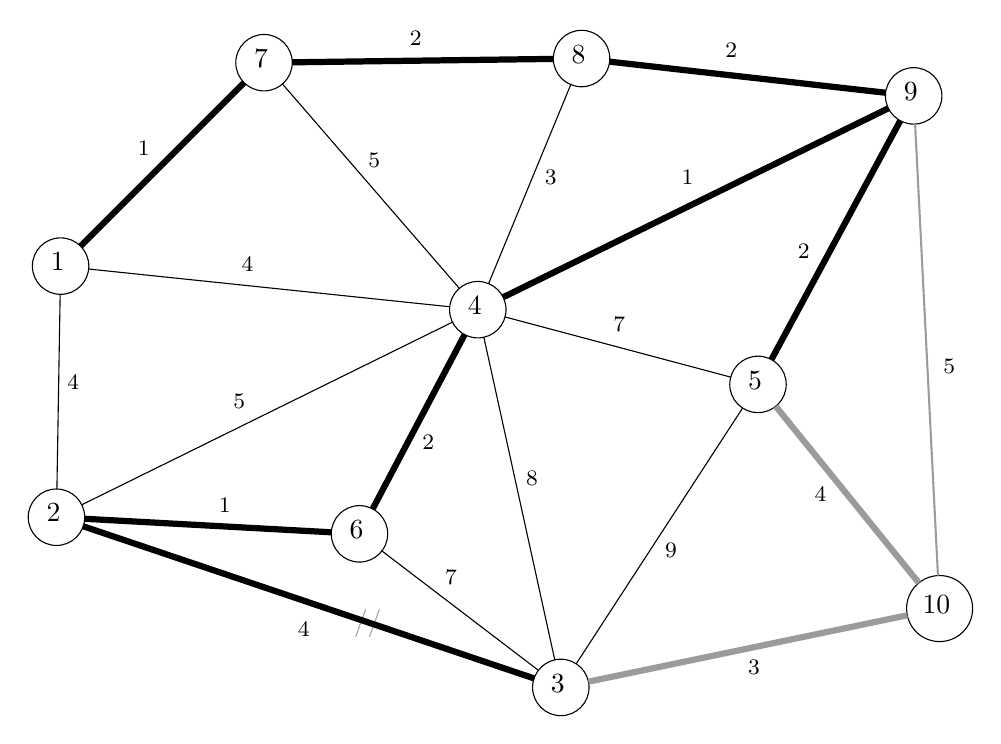
\begin{tikzpicture}[x=0.75pt,y=0.75pt,yscale=-1,xscale=1]
	%uncomment if require: \path (0,360); %set diagram left start at 0, and has height of 360


	% Text Node
	\draw    (38, 132) circle [x radius= 13.6, y radius= 13.6]   ;
	\draw (32,124.4) node [anchor=north west][inner sep=0.75pt]    {$1$};
	% Text Node
	\draw    (36, 253) circle [x radius= 13.6, y radius= 13.6]   ;
	\draw (30,245.4) node [anchor=north west][inner sep=0.75pt]    {$2$};
	% Text Node
	\draw    (279, 335) circle [x radius= 13.6, y radius= 13.6]   ;
	\draw (273,327.4) node [anchor=north west][inner sep=0.75pt]    {$3$};
	% Text Node
	\draw    (239, 153) circle [x radius= 13.6, y radius= 13.6]   ;
	\draw (233,145.4) node [anchor=north west][inner sep=0.75pt]    {$4$};
	% Text Node
	\draw    (374, 189) circle [x radius= 13.6, y radius= 13.6]   ;
	\draw (368,181.4) node [anchor=north west][inner sep=0.75pt]    {$5$};
	% Text Node
	\draw    (182, 261) circle [x radius= 13.6, y radius= 13.6]   ;
	\draw (176,253.4) node [anchor=north west][inner sep=0.75pt]    {$6$};
	% Text Node
	\draw    (136, 34) circle [x radius= 13.6, y radius= 13.6]   ;
	\draw (130,26.4) node [anchor=north west][inner sep=0.75pt]    {$7$};
	% Text Node
	\draw    (289, 32) circle [x radius= 13.6, y radius= 13.6]   ;
	\draw (283,24.4) node [anchor=north west][inner sep=0.75pt]    {$8$};
	% Text Node
	\draw    (449, 50) circle [x radius= 13.6, y radius= 13.6]   ;
	\draw (443,42.4) node [anchor=north west][inner sep=0.75pt]    {$9$};
	% Text Node
	\draw    (461.5, 297) circle [x radius= 15.91, y radius= 15.91]   ;
	\draw (452,289.4) node [anchor=north west][inner sep=0.75pt]    {$10$};
	% Text Node
	\draw (74,70.4) node [anchor=north west][inner sep=0.75pt]  [font=\footnotesize]  {$1$};
	% Text Node
	\draw (336,84.4) node [anchor=north west][inner sep=0.75pt]  [font=\footnotesize]  {$1$};
	% Text Node
	\draw (113,242.4) node [anchor=north west][inner sep=0.75pt]  [font=\footnotesize]  {$1$};
	% Text Node
	\draw (211,212.4) node [anchor=north west][inner sep=0.75pt]  [font=\footnotesize]  {$2$};
	% Text Node
	\draw (357,23.4) node [anchor=north west][inner sep=0.75pt]  [font=\footnotesize]  {$2$};
	% Text Node
	\draw (392,120.4) node [anchor=north west][inner sep=0.75pt]  [font=\footnotesize]  {$2$};
	% Text Node
	\draw (270,84.4) node [anchor=north west][inner sep=0.75pt]  [font=\footnotesize]  {$3$};
	% Text Node
	\draw (368,320.4) node [anchor=north west][inner sep=0.75pt]  [font=\footnotesize]  {$3$};
	% Text Node
	\draw (124,126.4) node [anchor=north west][inner sep=0.75pt]  [font=\footnotesize]  {$4$};
	% Text Node
	\draw (40,183.4) node [anchor=north west][inner sep=0.75pt]  [font=\footnotesize]  {$4$};
	% Text Node
	\draw (400,237.4) node [anchor=north west][inner sep=0.75pt]  [font=\footnotesize]  {$4$};
	% Text Node
	\draw (120,192.4) node [anchor=north west][inner sep=0.75pt]  [font=\footnotesize]  {$5$};
	% Text Node
	\draw (151,302.4) node [anchor=north west][inner sep=0.75pt]  [font=\footnotesize]  {$4$};
	% Text Node
	\draw (462,175.4) node [anchor=north west][inner sep=0.75pt]  [font=\footnotesize]  {$5$};
	% Text Node
	\draw (185,76.4) node [anchor=north west][inner sep=0.75pt]  [font=\footnotesize]  {$5$};
	% Text Node
	\draw (205,17.4) node [anchor=north west][inner sep=0.75pt]  [font=\footnotesize]  {$2$};
	% Text Node
	\draw (303,155.4) node [anchor=north west][inner sep=0.75pt]  [font=\footnotesize]  {$7$};
	% Text Node
	\draw (222,277.4) node [anchor=north west][inner sep=0.75pt]  [font=\footnotesize]  {$7$};
	% Text Node
	\draw (261,229.4) node [anchor=north west][inner sep=0.75pt]  [font=\footnotesize]  {$8$};
	% Text Node
	\draw (328,264.4) node [anchor=north west][inner sep=0.75pt]  [font=\footnotesize]  {$9$};
	% Text Node
	\draw (178,296.4) node [anchor=north west][inner sep=0.75pt]  [color={rgb, 255:red, 155; green, 155; blue, 155 }  ,opacity=1 ]  {$//$};
	% Connection
	\draw    (244.2,140.43) -- (283.8,44.57) ;
	% Connection
	\draw    (230.1,142.72) -- (144.9,44.28) ;
	% Connection
	\draw    (225.47,151.59) -- (51.53,133.41) ;
	% Connection
	\draw    (226.8,159.01) -- (48.2,246.99) ;
	% Connection
	\draw [line width=2.25]    (232.65,165.03) -- (188.35,248.97) ;
	% Connection
	\draw    (241.92,166.29) -- (276.08,321.71) ;
	% Connection
	\draw    (252.15,156.51) -- (360.85,185.49) ;
	% Connection
	\draw [line width=2.25]    (251.21,147.01) -- (436.79,55.99) ;
	% Connection
	\draw [line width=2.25]    (302.52,33.52) -- (435.48,48.48) ;
	% Connection
	\draw [line width=2.25]    (275.4,32.18) -- (149.6,33.82) ;
	% Connection
	\draw [line width=2.25]    (47.62,122.38) -- (126.38,43.62) ;
	% Connection
	\draw    (37.78,145.6) -- (36.22,239.4) ;
	% Connection
	\draw    (192.81,269.25) -- (268.19,326.75) ;
	% Connection
	\draw [line width=2.25]    (168.42,260.26) -- (49.58,253.74) ;
	% Connection
	\draw [line width=2.25]    (48.89,257.35) -- (266.11,330.65) ;
	% Connection
	\draw [line width=2.25]    (380.46,177.03) -- (442.54,61.97) ;
	% Connection
	\draw    (366.58,200.4) -- (286.42,323.6) ;
	% Connection
	\draw [color={rgb, 255:red, 155; green, 155; blue, 155 }  ,draw opacity=1 ][line width=2.25]    (382.56,199.57) -- (451.48,284.63) ;
	% Connection
	\draw [color={rgb, 255:red, 155; green, 155; blue, 155 }  ,draw opacity=1 ][line width=0.75]    (460.7,281.11) -- (449.69,63.58) ;
	% Connection
	\draw [color={rgb, 255:red, 155; green, 155; blue, 155 }  ,draw opacity=1 ][line width=2.25]    (445.92,300.24) -- (292.32,332.23) ;

	\end{tikzpicture}
\end{figure}
\FloatBarrier

\begin{equation*}
\begin{array}{ c c c c }
\text{Lato} & \text{Costo} & \text{Accettato} & | T| \\
( 1,7) & 1 & \text{\cmark}  & 1\\
( 2,6) & 1 & \text{\cmark}  & 2\\
( 4,9) & 1 & \text{\cmark}  & 3\\
( 4,6) & 2 & \text{\cmark}  & 4\\
( 5,9) & 2 & \text{\cmark}  & 5\\
( 8,9) & 2 & \text{\cmark}  & 6\\
( 7,8) & 2 & \text{\cmark}  & 7\\
( 8,4) & 3 & \text{\xmark}  & \\
\textcolor[rgb]{0.61,0.61,0.61}{( 3,10)} & \textcolor[rgb]{0.61,0.61,0.61}{3} & \text{\textcolor[rgb]{0.61,0.61,0.61}{\cmark }} & \textcolor[rgb]{0.61,0.61,0.61}{8}\\
( 1,4) & 4 & \text{\xmark \textcolor[rgb]{0.61,0.61,0.61}{\xmark }} & \\
( 2,1) & 4 & \text{\xmark \textcolor[rgb]{0.61,0.61,0.61}{\xmark }} & \\
\textcolor[rgb]{0.61,0.61,0.61}{( 5,10}\textcolor[rgb]{0.61,0.61,0.61}{)} & \textcolor[rgb]{0.61,0.61,0.61}{4} & \text{\textcolor[rgb]{0.61,0.61,0.61}{\cmark }} & \textcolor[rgb]{0.61,0.61,0.61}{9\ \text{(stop!)}}\\
( 2,3) & 4 & \text{\cmark}  & 8\\
\textcolor[rgb]{0.61,0.61,0.61}{( 4,10}\textcolor[rgb]{0.61,0.61,0.61}{)} & \textcolor[rgb]{0.61,0.61,0.61}{5} &  & \\
( 7,4) & 5 &  & \\
( 2,4) & 5 &  & \\
( 4,5) & 7 &  & \\
( 6,3) & 7 &  & \\
( 4,3) & 8 &  & \\
( 3,5) & 9 &  & 
\end{array}
\end{equation*}
%!TEX root = ../fro.tex
\chapter{Programmazione Lineare Intera}

\Es
\begin{gather*}
x_{2} \leq \frac{1}{5} x_{1} +4\\
x_{2} \leq -2x_{1} +\frac{19}{2}\\
x_{2} \geq x_{1} -1
\end{gather*}

\begin{figure}[htpb]
	\centering
	\tikzset{every picture/.style={line width=0.75pt}} %set default line width to 0.75pt        

	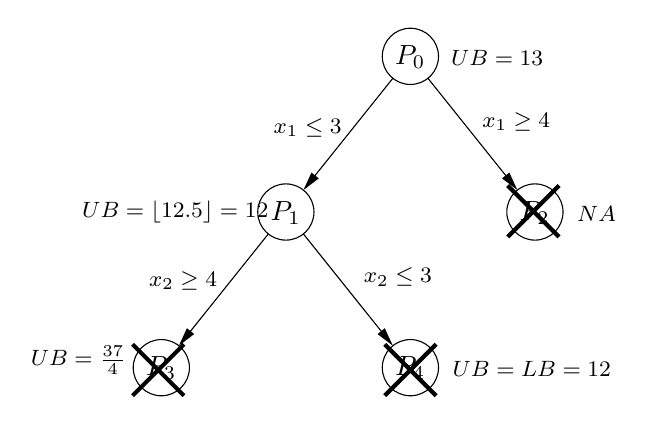
\begin{tikzpicture}[x=0.75pt,y=0.75pt,yscale=-0.75,xscale=0.75]
	%uncomment if require: \path (0,340); %set diagram left start at 0, and has height of 340

	%Straight Lines [id:da8256496838848162] 
	\draw [line width=1.5]    (355,146) -- (388,179) ;
	%Straight Lines [id:da14854697063972377] 
	\draw [line width=1.5]    (388,146) -- (355,179) ;
	%Straight Lines [id:da038487184733093205] 
	\draw [line width=1.5]    (276,248) -- (309,281) ;
	%Straight Lines [id:da09421605800632826] 
	\draw [line width=1.5]    (309,248) -- (276,281) ;
	%Straight Lines [id:da7070304946661545] 
	\draw [line width=1.5]    (114,248) -- (147,281) ;
	%Straight Lines [id:da48001648506360284] 
	\draw [line width=1.5]    (147,248) -- (114,281) ;

	% Text Node
	\draw    (292.5, 63) circle [x radius= 18.06, y radius= 18.06]   ;
	\draw (281,54.4) node [anchor=north west][inner sep=0.75pt]    {$P_{0}$};
	% Text Node
	\draw    (212.5, 163) circle [x radius= 18.06, y radius= 18.06]   ;
	\draw (201,154.4) node [anchor=north west][inner sep=0.75pt]    {$P_{1}$};
	% Text Node
	\draw    (372.5, 163) circle [x radius= 18.06, y radius= 18.06]   ;
	\draw (361,154.4) node [anchor=north west][inner sep=0.75pt]    {$P_{2}$};
	% Text Node
	\draw    (132.5, 263) circle [x radius= 18.06, y radius= 18.06]   ;
	\draw (121,254.4) node [anchor=north west][inner sep=0.75pt]    {$P_{3}$};
	% Text Node
	\draw    (292.5, 263) circle [x radius= 18.06, y radius= 18.06]   ;
	\draw (281,254.4) node [anchor=north west][inner sep=0.75pt]    {$P_{4}$};
	% Text Node
	\draw (317,57.4) node [anchor=north west][inner sep=0.75pt]  [font=\footnotesize]  {$UB=13$};
	% Text Node
	\draw (80,154.4) node [anchor=north west][inner sep=0.75pt]  [font=\footnotesize]  {$UB=\lfloor 12.5\rfloor =12$};
	% Text Node
	\draw (398,157.4) node [anchor=north west][inner sep=0.75pt]  [font=\footnotesize]  {$NA$};
	% Text Node
	\draw (318,257.4) node [anchor=north west][inner sep=0.75pt]  [font=\footnotesize]  {$UB=LB=12$};
	% Text Node
	\draw (47,247.4) node [anchor=north west][inner sep=0.75pt]  [font=\footnotesize]  {$UB=\frac{37}{4}$};
	% Text Node
	\draw (337,97.4) node [anchor=north west][inner sep=0.75pt]  [font=\footnotesize]  {$x_{1} \geq 4$};
	% Text Node
	\draw (203,101.4) node [anchor=north west][inner sep=0.75pt]  [font=\footnotesize]  {$x_{1} \leq 3$};
	% Text Node
	\draw (261,197.4) node [anchor=north west][inner sep=0.75pt]  [font=\footnotesize]  {$x_{2} \leq 3$};
	% Text Node
	\draw (123,199.4) node [anchor=north west][inner sep=0.75pt]  [font=\footnotesize]  {$x_{2} \geq 4$};
	% Connection
	\draw    (281.22,77.1) -- (225.03,147.33) ;
	\draw [shift={(223.78,148.9)}, rotate = 308.66] [fill={rgb, 255:red, 0; green, 0; blue, 0 }  ][line width=0.08]  [draw opacity=0] (12,-3) -- (0,0) -- (12,3) -- cycle    ;
	% Connection
	\draw    (303.78,77.1) -- (359.97,147.33) ;
	\draw [shift={(361.22,148.9)}, rotate = 231.34] [fill={rgb, 255:red, 0; green, 0; blue, 0 }  ][line width=0.08]  [draw opacity=0] (12,-3) -- (0,0) -- (12,3) -- cycle    ;
	% Connection
	\draw    (201.22,177.1) -- (145.03,247.33) ;
	\draw [shift={(143.78,248.9)}, rotate = 308.66] [fill={rgb, 255:red, 0; green, 0; blue, 0 }  ][line width=0.08]  [draw opacity=0] (12,-3) -- (0,0) -- (12,3) -- cycle    ;
	% Connection
	\draw    (223.78,177.1) -- (279.97,247.33) ;
	\draw [shift={(281.22,248.9)}, rotate = 231.34] [fill={rgb, 255:red, 0; green, 0; blue, 0 }  ][line width=0.08]  [draw opacity=0] (12,-3) -- (0,0) -- (12,3) -- cycle    ;

	\end{tikzpicture}
\end{figure}
\FloatBarrier

Ottimo: $12,( 3,3)$.

\begin{figure}
\centering
\begin{subfigure}{.5\textwidth}
  \centering
  \includegraphics[width=\linewidth]{1-1}
\end{subfigure}%
\begin{subfigure}{.5\textwidth}
  \centering
  \includegraphics[width=\linewidth]{1-2}
\end{subfigure}
\end{figure}
\FloatBarrier

\Es

\begin{figure}[htpb]
	\centering
	\tikzset{every picture/.style={line width=0.75pt}} %set default line width to 0.75pt        

	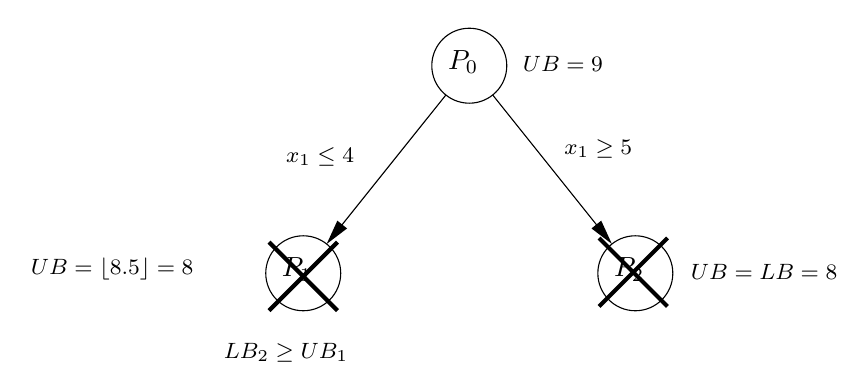
\begin{tikzpicture}[x=0.75pt,y=0.75pt,yscale=-1,xscale=1]
	%uncomment if require: \path (0,255); %set diagram left start at 0, and has height of 255

	%Straight Lines [id:da31633087052970965] 
	\draw [line width=1.5]    (355,146) -- (388,179) ;
	%Straight Lines [id:da4125010004484957] 
	\draw [line width=1.5]    (388,146) -- (355,179) ;
	%Straight Lines [id:da7570488418846992] 
	\draw [line width=1.5]    (196,148) -- (229,181) ;
	%Straight Lines [id:da8927568555222583] 
	\draw [line width=1.5]    (229,148) -- (196,181) ;

	% Text Node
	\draw    (292.5, 63) circle [x radius= 18.06, y radius= 18.06]   ;
	\draw (281,54.4) node [anchor=north west][inner sep=0.75pt]    {$P_{0}$};
	% Text Node
	\draw    (212.5, 163) circle [x radius= 18.06, y radius= 18.06]   ;
	\draw (201,154.4) node [anchor=north west][inner sep=0.75pt]    {$P_{1}$};
	% Text Node
	\draw    (372.5, 163) circle [x radius= 18.06, y radius= 18.06]   ;
	\draw (361,154.4) node [anchor=north west][inner sep=0.75pt]    {$P_{2}$};
	% Text Node
	\draw (317,57.4) node [anchor=north west][inner sep=0.75pt]  [font=\footnotesize]  {$UB=9$};
	% Text Node
	\draw (80,154.4) node [anchor=north west][inner sep=0.75pt]  [font=\footnotesize]  {$UB=\lfloor 8.5\rfloor =8$};
	% Text Node
	\draw (398,157.4) node [anchor=north west][inner sep=0.75pt]  [font=\footnotesize]  {$UB=LB=8$};
	% Text Node
	\draw (337,97.4) node [anchor=north west][inner sep=0.75pt]  [font=\footnotesize]  {$x_{1} \geq 5$};
	% Text Node
	\draw (203,101.4) node [anchor=north west][inner sep=0.75pt]  [font=\footnotesize]  {$x_{1} \leq 4$};
	% Text Node
	\draw (173,195.4) node [anchor=north west][inner sep=0.75pt]  [font=\footnotesize]  {$LB_{2} \geq UB_{1}$};
	% Connection
	\draw    (281.22,77.1) -- (225.03,147.33) ;
	\draw [shift={(223.78,148.9)}, rotate = 308.66] [fill={rgb, 255:red, 0; green, 0; blue, 0 }  ][line width=0.08]  [draw opacity=0] (12,-3) -- (0,0) -- (12,3) -- cycle    ;
	% Connection
	\draw    (303.78,77.1) -- (359.97,147.33) ;
	\draw [shift={(361.22,148.9)}, rotate = 231.34] [fill={rgb, 255:red, 0; green, 0; blue, 0 }  ][line width=0.08]  [draw opacity=0] (12,-3) -- (0,0) -- (12,3) -- cycle    ;

	\end{tikzpicture}
\end{figure}
\FloatBarrier

Ottimo: $8,( 5,-1)$.

\fg{0.5}{2}

\Es

Rilassamento continuo:
\begin{equation*}
x_{1} =0\ \ x_{2} =\frac{7}{2} \ \ s_{1} =0\ \ s_{2} =\frac{3}{2}
\end{equation*}
Equazioni dei tagli:
\begin{equation*}
\begin{array}{ l l l l l c }
x_{2} +x_{1} +\frac{1}{2} s_{1} =\frac{7}{2} & \rightarrow  & x_{2} +x_{1} +\left\lfloor \frac{1}{2}\right\rfloor s_{1} \leq \left\lfloor \frac{7}{2}\right\rfloor  & \rightarrow  & x_{2} +x_{1} \leq 3 & \boxed{x_{1} +x_{2} \leq 3}\\
s_{2} -x_{1} +\frac{1}{2} s_{1} =\frac{3}{2} & \rightarrow  & s_{2} -x_{1} +\left\lfloor \frac{1}{2}\right\rfloor s_{1} \leq \left\lfloor \frac{3}{2}\right\rfloor  & \rightarrow  & s_{2} -x_{1} \leq 1 & \\
 &  &  &  & s_{2} =2x_{1} +x_{2} -2 & 
\end{array}
\end{equation*}
Ottimo: $-6,( 0,3)$.

\fg{0.3}{3}

\Es

Rilassamento continuo:
\begin{equation*}
x_{1} =0\ \ x_{2} =\frac{9}{2} \ \ s_{1} =0\ \ s_{2} =\frac{5}{2}
\end{equation*}
Equazioni dei tagli:
\begin{equation*}
\begin{array}{ l l l l l c }
x_{2} +\frac{1}{2} s_{1} =\frac{9}{2} & \rightarrow  & x_{2} +\left\lfloor \frac{1}{2}\right\rfloor s_{1} \leq \left\lfloor \frac{9}{2}\right\rfloor  & \rightarrow  & x_{2} \leq 4 & \boxed{x_{2} \leq 4}\\
s_{2} +2x_{1} -\frac{1}{2} s_{1} =\frac{5}{2} & \rightarrow  & s_{2} +2x_{1} -\left\lfloor \frac{1}{2}\right\rfloor s_{1} \leq \left\lfloor \frac{5}{2}\right\rfloor  & \rightarrow  & s_{2} +2x_{1} -s_{1} \leq 2 & 
\end{array}
\end{equation*}
Ottimo: $-8,( 0,4)$.

\fg{0.6}{4}

\Es

$B=13$.
\begin{equation*}
\arraycolsep=2pt\def\arraystretch{1.6}
\begin{array}{ c|c c c c }
p_{i} & 16 & 9 & 12 & 2\\
\hline
w_{i} & 8 & 6 & 7 & 2\\
\hline
\frac{p_{i}}{w_{i}} & 2 & \frac{3}{2} & \frac{12}{7} & 1\\
\hline
 & x_{1} & x_{2} & x_{3} & x_{4}
\end{array}
\end{equation*}
Ordino
\begin{equation*}
x_{1} ,x_{3} ,x_{2} ,x_{4}
\end{equation*}

\begin{figure}[htpb]
	\centering
	\tikzset{every picture/.style={line width=0.75pt}} %set default line width to 0.75pt        

	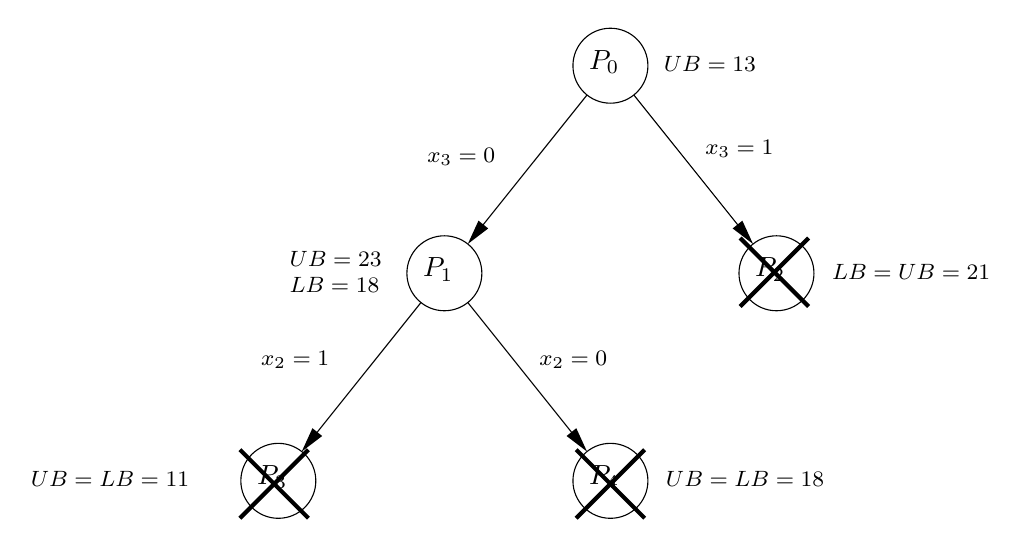
\begin{tikzpicture}[x=0.75pt,y=0.75pt,yscale=-1,xscale=1]
	%uncomment if require: \path (0,340); %set diagram left start at 0, and has height of 340

	%Straight Lines [id:da902458193250876] 
	\draw [line width=1.5]    (355,146) -- (388,179) ;
	%Straight Lines [id:da770061225974817] 
	\draw [line width=1.5]    (388,146) -- (355,179) ;
	%Straight Lines [id:da6732168860960122] 
	\draw [line width=1.5]    (276,248) -- (309,281) ;
	%Straight Lines [id:da5913463822053582] 
	\draw [line width=1.5]    (309,248) -- (276,281) ;
	%Straight Lines [id:da8203822268133403] 
	\draw [line width=1.5]    (114,248) -- (147,281) ;
	%Straight Lines [id:da5206633509023615] 
	\draw [line width=1.5]    (147,248) -- (114,281) ;

	% Text Node
	\draw    (292.5, 63) circle [x radius= 18.06, y radius= 18.06]   ;
	\draw (281,54.4) node [anchor=north west][inner sep=0.75pt]    {$P_{0}$};
	% Text Node
	\draw    (212.5, 163) circle [x radius= 18.06, y radius= 18.06]   ;
	\draw (201,154.4) node [anchor=north west][inner sep=0.75pt]    {$P_{1}$};
	% Text Node
	\draw    (372.5, 163) circle [x radius= 18.06, y radius= 18.06]   ;
	\draw (361,154.4) node [anchor=north west][inner sep=0.75pt]    {$P_{2}$};
	% Text Node
	\draw    (132.5, 263) circle [x radius= 18.06, y radius= 18.06]   ;
	\draw (121,254.4) node [anchor=north west][inner sep=0.75pt]    {$P_{3}$};
	% Text Node
	\draw    (292.5, 263) circle [x radius= 18.06, y radius= 18.06]   ;
	\draw (281,254.4) node [anchor=north west][inner sep=0.75pt]    {$P_{4}$};
	% Text Node
	\draw (317,57.4) node [anchor=north west][inner sep=0.75pt]  [font=\footnotesize]  {$UB=13$};
	% Text Node
	\draw (130,149.4) node [anchor=north west][inner sep=0.75pt]  [font=\footnotesize]  {$ \begin{array}{l}
	UB=23\\
	LB=18
	\end{array}$};
	% Text Node
	\draw (398,157.4) node [anchor=north west][inner sep=0.75pt]  [font=\footnotesize]  {$LB=UB=21$};
	% Text Node
	\draw (318,257.4) node [anchor=north west][inner sep=0.75pt]  [font=\footnotesize]  {$UB=LB=18$};
	% Text Node
	\draw (12,257.4) node [anchor=north west][inner sep=0.75pt]  [font=\footnotesize]  {$UB=LB=11$};
	% Text Node
	\draw (337,97.4) node [anchor=north west][inner sep=0.75pt]  [font=\footnotesize]  {$x_{3} =1$};
	% Text Node
	\draw (203,101.4) node [anchor=north west][inner sep=0.75pt]  [font=\footnotesize]  {$x_{3} =0$};
	% Text Node
	\draw (257,199.4) node [anchor=north west][inner sep=0.75pt]  [font=\footnotesize]  {$x_{2} =0$};
	% Text Node
	\draw (123,199.4) node [anchor=north west][inner sep=0.75pt]  [font=\footnotesize]  {$x_{2} =1$};
	% Connection
	\draw    (281.22,77.1) -- (225.03,147.33) ;
	\draw [shift={(223.78,148.9)}, rotate = 308.66] [fill={rgb, 255:red, 0; green, 0; blue, 0 }  ][line width=0.08]  [draw opacity=0] (12,-3) -- (0,0) -- (12,3) -- cycle    ;
	% Connection
	\draw    (303.78,77.1) -- (359.97,147.33) ;
	\draw [shift={(361.22,148.9)}, rotate = 231.34] [fill={rgb, 255:red, 0; green, 0; blue, 0 }  ][line width=0.08]  [draw opacity=0] (12,-3) -- (0,0) -- (12,3) -- cycle    ;
	% Connection
	\draw    (201.22,177.1) -- (145.03,247.33) ;
	\draw [shift={(143.78,248.9)}, rotate = 308.66] [fill={rgb, 255:red, 0; green, 0; blue, 0 }  ][line width=0.08]  [draw opacity=0] (12,-3) -- (0,0) -- (12,3) -- cycle    ;
	% Connection
	\draw    (223.78,177.1) -- (279.97,247.33) ;
	\draw [shift={(281.22,248.9)}, rotate = 231.34] [fill={rgb, 255:red, 0; green, 0; blue, 0 }  ][line width=0.08]  [draw opacity=0] (12,-3) -- (0,0) -- (12,3) -- cycle    ;

	\end{tikzpicture}
\end{figure}
\FloatBarrier

$P_{0}$:
\begin{align*}
x_{1} & =1\ \ \ \ \overline{B} =5\\
x_{3} & =\frac{5}{7} \ \ \ \ \overline{B} =0\\
x_{2} ,x_{4} & =0\\
UB_{0} & =\left\lfloor 16+\frac{60}{7}\right\rfloor =24\\
LB_{0} & =16+2=18
\end{align*}
$P_{1}$:
\begin{align*}
x_{3} & =0\ \ \ \ \overline{B} =13\\
x_{1} & =1\ \ \ \ \overline{B} =5\\
x_{2} & =\frac{5}{6} \ \ \ \ \overline{B} =0\\
UB_{1} & =\left\lfloor 16+\frac{45}{6}\right\rfloor =23\\
LB_{1} & =16+2=18
\end{align*}
$P_{2}$:
\begin{align*}
x_{3} & =1\ \ \ \ \overline{B} =6\\
x_{1} & =0\ \ \ \ \overline{B} =6\\
x_{2} & =1\ \ \ \ \overline{B} =0\\
UB_{2} & =LB_{2} =21
\end{align*}
$P_{3}$:
\begin{align*}
x_{3} & =0\ \ \ \ \overline{B} =7\\
x_{2} & =1\ \ \ \ \overline{B} =7\\
x_{1} & =0\ \ \ \ \overline{B} =7\\
x_{4} & =1\ \ \ \ \overline{B} =5\\
UB_{3} & =LB_{3} =11
\end{align*}
$P_{4}$:
\begin{align*}
x_{2} & =0\ \ \ \ \overline{B} =13\\
x_{3} & =0\ \ \ \ \overline{B} =13\\
x_{1} & =1\ \ \ \ \overline{B} =5\\
x_{4} & =1\ \ \ \ \overline{B} =3\\
UB_{4} & =LB_{4} =18
\end{align*}

\chapter*{Schema esercizi}
Lo schema seguente è incredibilmente utile, tuttavia non siamo riusciti a trovare la voglia di finirlo, aiutateci.
\includepdf[noautoscale=true, width=\paperwidth, pages=-]{chapters/schema.pdf}

\end{document}